\spacing{1.3}

\section{Introduction}
The word \textbf{atom} was first introduced by Greek philosophers over 2000 years ago and means \textbf{indivisible}, that is, something that cannot be divided into smaller parts.

The atom is extraordinarily small. To give you an idea of its size: if an atom were the size of a marble, a real marble would be the size of the Earth. The hydrogen atom, which is the smallest of all, has a size on the order of \qty{e-10}{\metre} (this is one ten-billionth of a meter!).
\begin{remark}
    \textbf{Did you know...?} If we lined up atoms in a row, we would need approximately 10 million atoms to cover the thickness of a sheet of paper.
\end{remark}
All the matter around us is made up of atoms: the air we breathe, the water we drink, our own bodies... For this reason, throughout history, different scientists have dedicated their lives to trying to understand what atoms are like and how they are formed.
\section{Atomic Model}
\begin{definition}[Atomic model]
    It is the representation of the atom in which its parts and how they are organized are identified. It is like a ``map'' that helps us understand something that is too small to see directly.
\end{definition}
\subsection{The Particles of the Atom}

Although the name ``atom'' means indivisible, today we know that atoms do have parts. The atom is made up of three types of fundamental particles:
\begin{itemize}
    \item \negsubro{Protons (\prt{}):} are particles with a \textbf{positive electric charge} (+). We can imagine them as small balls with a ``+'' sign.
    \item \negsubro{Neutrons (\ntr{}):} are particles \textbf{with no electric charge}. They are ``neutral,'' hence their name.
    \item \negsubro{Electrons (\el{}):} are particles with a \textbf{negative electric charge} (-). They are much smaller and lighter than protons and neutrons.
\end{itemize}
\begin{remark}
    \prt{} and \ntr{} have a similar mass (they are like twins in terms of size), while \el{} are much lighter. If a proton weighed 1 kg, an electron would weigh barely 0.5 grams. Almost 2000 times less!
\end{remark}
\subsection{Structure of the Atom}
The atom is organized into two distinct zones:
\begin{itemize}
    \item \negsubro{Nucleus}. It is the center of the atom, like the heart of a city. Here the \textbf{protons and neutrons} are found very close together and compact. Although the nucleus is very small compared to the total size of the atom, it contains almost all of its mass.
    \item \negsubro{Electron cloud}. It is the zone that surrounds the nucleus, like the outskirts of a city. Here the \textbf{electrons} are found moving at high speed around the nucleus. Electrons do not move randomly, but rather occupy specific zones called \textbf{orbitals}, which are like ``highways'' where they can move.
\end{itemize}
\begin{remark}
    \textbf{An interesting comparison:} If the nucleus of an atom were the size of a tennis ball placed in the center of a soccer stadium, the electrons would be circling around the stands. The atom is mostly empty space!
\end{remark}
\subsection{Atoms Are Neutral}
Under normal conditions, atoms are \textbf{electrically neutral}, that is, they have no total electric charge. This occurs because they have the same number of positive charges (protons) as negative charges (electrons), and they balance each other out.

Therefore, in a \textbf{neutral atom} we will have: \(\text{Number of protons} = \text{Number of electrons}\)

\section{Atomic Number and Mass Number}

To identify and differentiate the different types of atoms, scientists use two very important numbers: the \textbf{atomic number} and the \textbf{mass number}.

\subsection{Atomic Number (Z)}

The \textbf{atomic number}, symbolized by the letter \( \bm{Z} \), indicates the \textbf{number of protons} that an atom has in its nucleus.
\begin{centeredequation}
    Z = \text{number of protons}
\end{centeredequation}
The atomic number is like the ``ID card'' of each chemical element. It is what defines which element an atom belongs to:
\begin{itemize}
    \item All hydrogen atoms have \( Z = 1 \) (1 proton)
    \item All carbon atoms have \( Z = 6 \) (6 protons)
    \item All oxygen atoms have \( Z = 8 \) (8 protons)
\end{itemize}
\begin{remark}
    As we have already seen, in a neutral atom the number of protons equals the number of electrons. Therefore, the atomic number also tells us how many electrons it has: \( \el{} = Z \)
\end{remark}
\subsection{Mass Number (A)}
The \textbf{mass number}, symbolized by the letter \( \bm{A} \), indicates the \textbf{total number of particles} in the nucleus (protons + neutrons).
\begin{centeredequation}
    A = \text{number of protons} + \text{number of neutrons}
\end{centeredequation}

\subsection{Calculating the Number of Neutrons}

If we know the mass number (\( A \)) and the atomic number (\( Z \)), we can easily calculate how many neutrons an atom has:
\begin{centeredequation}
    \text{Number of neutrons} = A - Z
\end{centeredequation}
\begin{remark}
    \textbf{Why?} Because if \( A \) is the sum of protons and neutrons, and \( Z \) is the number of protons, by subtracting we obtain only the neutrons.
\end{remark}
\subsection{Representation of Atoms}
\begin{minipage}{0.45\textwidth}
    Elements are represented by indicating the element symbol, the atomic number, and the mass number, as shown in the Figure \ref{fig:massatomic}
    \begin{remark}
        If no \( + \) or \( - \) sign appears in the \blueremark{upper right} of the element symbol, this indicates that the atom is \textbf{neutral} and therefore has the same number of protons as electrons.
    \end{remark}
\end{minipage}
\hfill
\begin{minipage}{0.45\textwidth}
    \begin{figure}[H]
        \centering
%        \includegraphics[scale=0.6]{images/SP_atomo/z_a_atomica_figura.pdf}
        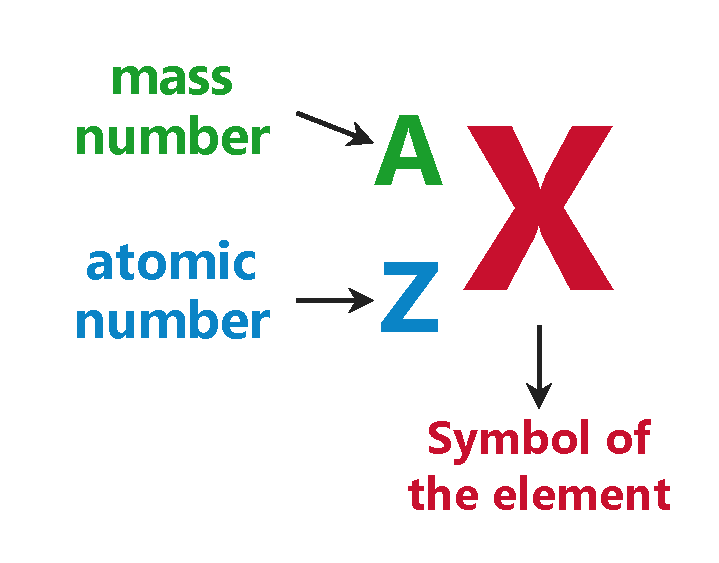
\includegraphics[width=0.8\linewidth]{Figuras_SVG_ENG/pdf/U6_numero_masico_atomico.pdf}
        \caption{Representation of mass number and atomic number}
        \label{fig:massatomic}
    \end{figure}
\end{minipage}
%\begin{figure}[H]
%    \centering
%    \includegraphics[scale=0.6]{images/SP_atomo/z_a_atomica_figura.pdf}
%    \caption{Representation of mass number and atomic number}
%    \label{fig:massatomic}
%\end{figure}
\begin{example}
    Let's determine the number of protons, neutrons, and electrons in the following neutral atoms:
    \begin{itemize}
        \item \textbf{\isotope{Na} (Sodium):}
        \begin{itemize}
            \item Protons: \( Z = 11 \) → 11 protons
            \item Electrons: Since it is neutral, 11 electrons
            \item Neutrons: \( \ntr = A - Z = 23 - 11 = 12 \) neutrons
        \end{itemize}

        \item \textbf{\isotope{Po} (Polonium):}
        \begin{itemize}
            \item Protons: \( Z = 84 \) → 84 protons
            \item Electrons: Since it is neutral, 84 electrons
            \item Neutrons: \( \ntr = A - Z = 209 - 84 = 125 \) neutrons
        \end{itemize}
    \end{itemize}
\end{example}


\begin{exercise}
    Indicate the number of protons, neutrons, and electrons in a chlorine atom \isotope{Cl}.

    \begin{solu}
        To solve this exercise, we need to interpret the isotopic notation of chlorine.

        From the notation \isotope{Cl} we obtain:
        \begin{itemize}
            \item Mass number (A) = 35 (upper part)
            \item Atomic number (Z) = 17 (lower part)
        \end{itemize}

        \textbf{Step 1: Calculate the number of protons}

        The atomic number (Z) directly indicates the number of protons:
        \[
            \text{Number of protons} = Z = 17
        \]

        \textbf{Step 2: Calculate the number of neutrons}

        The number of neutrons is calculated by subtracting the atomic number from the mass number:
        \[
            \text{Number of neutrons} = A - Z = 35 - 17 = 18
        \]

        \textbf{Step 3: Calculate the number of electrons}

        Since the exercise indicates it is an atom (not an ion), it is electrically neutral. Therefore, the number of electrons equals the number of protons:
        \[
            \text{Number of electrons} = Z = 17
        \]

        \textbf{Answer:} The chlorine-35 atom has \textbf{17 protons, 18 neutrons, and 17 electrons}.
    \end{solu}
\end{exercise}
\begin{exercise}
    How would you represent an electrically neutral potassium atom if Z = 19 and A = 39? How many protons, neutrons, and electrons does it have?
    \begin{solu}
        \textbf{Step 1: Representation of the atom}

        To represent an atom we use the notation \ch{^{A}_{Z}X}, where:
        \begin{itemize}
            \item X = element symbol (K for potassium)
            \item A = mass number = 39
            \item Z = atomic number = 19
        \end{itemize}

        Therefore, the representation is: \ch{^{39}_{19}K}

        \textbf{Step 2: Calculate the number of protons}

        The number of protons equals the atomic number:
        \[
            \text{Number of protons} = Z = 19
        \]

        \textbf{Step 3: Calculate the number of neutrons}

        The number of neutrons is obtained by subtracting:
        \[
            \text{Number of neutrons} = A - Z = 39 - 19 = 20
        \]

        \textbf{Step 4: Calculate the number of electrons}

        Since the atom is electrically neutral (has no charge), the number of electrons equals the number of protons:
        \[
            \text{Number of electrons} = 19
        \]

        \textbf{Answer:} The atom is represented as \ch{^{39}_{19}K} and has \textbf{19 protons, 20 neutrons, and 19 electrons}.
    \end{solu}
\end{exercise}

\begin{exercise}
    Can we say that Z always indicates the number of electrons? Explain your answer.
    \begin{solu}
        \textbf{Concept analysis:}

        The atomic number (Z) is a property that defines the chemical element and represents the number of protons in the atom's nucleus. This value is constant for each element.

        \textbf{Case 1: Neutral atom}

        In an electrically neutral atom, the positive charge of the protons must be exactly compensated by the negative charge of the electrons. Therefore:
        \[
            \text{Number of electrons} = \text{Number of protons} = Z
        \]

        In this case, we \textbf{can} say that Z indicates the number of electrons.

        \textbf{Case 2: Ions (charged atoms)}

        When an atom gains or loses electrons, it becomes an ion:
        \begin{itemize}
            \item \textbf{Cation} (positive charge): has lost electrons
            \[
                \text{Number of electrons} = Z - \text{positive charge}
            \]
            Example: \ch{Na^{+}} has Z = 11, but only 10 electrons.

            \item \textbf{Anion} (negative charge): has gained electrons
            \[
                \text{Number of electrons} = Z + \text{negative charge}
            \]
            Example: \ch{Cl^{-}} has Z = 17, but 18 electrons.
        \end{itemize}

        In these cases, Z \textbf{does not} indicate the number of electrons.

        \textbf{Answer:} Not always. Z indicates the number of protons, which equals the number of electrons ONLY if the atom is neutral. If the atom has a charge (is an ion), the number of electrons will be different from the value of Z.
    \end{solu}
\end{exercise}
\begin{exercise}
    The number of neutrons in lithium is one more than the number of protons. Knowing that its mass number is 7:
    \begin{enumerate}[label=\letraminuscula]
    \item What is its atomic number?
    \item How many electrons does an electrically neutral lithium atom have?
    \end{enumerate}
    \begin{solu}
        \textbf{Given data:}
        \begin{itemize}
            \item Mass number: A = 7
            \item Relationship: number of neutrons = number of protons + 1
        \end{itemize}

        \textbf{Part a) Calculate the atomic number}

        \textbf{Step 1:} Express the relationship between neutrons and protons

        If we call Z the number of protons:
        \[
            \text{Number of neutrons} = Z + 1
        \]

        \textbf{Step 2:} Use the mass number relationship

        We know that the mass number is the sum of protons and neutrons:
        \[
            A = \text{protons} + \text{neutrons}
        \]
        \[
            7 = Z + (Z + 1)
        \]

        \textbf{Step 3:} Solve the equation
        \[
            7 = 2Z + 1
        \]
        \[
            6 = 2Z
        \]
        \[
            Z = 3
        \]

        \textbf{Answer a):} The atomic number of lithium is \textbf{Z = 3}.

        \textbf{Part b) Calculate the number of electrons}

        Since the exercise indicates that the atom is electrically neutral, the number of electrons must equal the number of protons so that the charges balance:
        \[
            \text{Number of electrons} = Z = 3
        \]

        \textbf{Answer b):} An electrically neutral lithium atom has \textbf{3 electrons}.

        \textbf{Verification:}
        \begin{itemize}
            \item Protons: 3
            \item Neutrons: 3 + 1 = 4
            \item Mass number: 3 + 4 = 7 \( \checkmark \)
        \end{itemize}
    \end{solu}
\end{exercise}
\begin{exercise}
    Represent in the notation \ch{^{A}_{Z}X} indicating the number of protons, neutrons, and electrons of the following atoms:
    \begin{multicols}{2}
        \begin{enumerate}[label=\letraminuscula]
    \item Boron with 5 protons and 6 neutrons
    \item Nitrogen with 7 protons and 7 neutrons
    \item Carbon with 6 protons and 6 neutrons
    \item Oxygen with 8 protons and 8 neutrons
    \item Fluorine with 9 protons and 10 neutrons
    \item Helium with 2 protons and 2 neutrons
        \end{enumerate}
    \end{multicols}
    \begin{solu}
        For each atom we will follow these steps:
        \begin{enumerate}
            \item Identify Z (number of protons)
            \item Calculate A (mass number = protons + neutrons)
            \item Determine the element symbol
            \item Calculate electrons (equal to protons if the atom is neutral)
        \end{enumerate}

        \textbf{a) Boron with 5 protons and 6 neutrons}
        \begin{itemize}
            \item Z = 5 (protons)
            \item A = 5 + 6 = 11
            \item Symbol: B
            \item Electrons = 5 (neutral atom)
        \end{itemize}
        Representation: \ch{^{11}_{5}B}

        \textbf{Answer:} \ch{^{11}_{5}B} has 5 protons, 6 neutrons, and 5 electrons.

        \textbf{b) Nitrogen with 7 protons and 7 neutrons}
        \begin{itemize}
            \item Z = 7 (protons)
            \item A = 7 + 7 = 14
            \item Symbol: N
            \item Electrons = 7 (neutral atom)
        \end{itemize}
        Representation: \ch{^{14}_{7}N}

        \textbf{Answer:} \ch{^{14}_{7}N} has 7 protons, 7 neutrons, and 7 electrons.

        \textbf{c) Carbon with 6 protons and 6 neutrons}
        \begin{itemize}
            \item Z = 6 (protons)
            \item A = 6 + 6 = 12
            \item Symbol: C
            \item Electrons = 6 (neutral atom)
        \end{itemize}
        Representation: \ch{^{12}_{6}C}

        \textbf{Answer:} \ch{^{12}_{6}C} has 6 protons, 6 neutrons, and 6 electrons.

        \textbf{d) Oxygen with 8 protons and 8 neutrons}
        \begin{itemize}
            \item Z = 8 (protons)
            \item A = 8 + 8 = 16
            \item Symbol: O
            \item Electrons = 8 (neutral atom)
        \end{itemize}
        Representation: \ch{^{16}_{8}O}

        \textbf{Answer:} \ch{^{16}_{8}O} has 8 protons, 8 neutrons, and 8 electrons.

        \textbf{e) Fluorine with 9 protons and 10 neutrons}
        \begin{itemize}
            \item Z = 9 (protons)
            \item A = 9 + 10 = 19
            \item Symbol: F
            \item Electrons = 9 (neutral atom)
        \end{itemize}
        Representation: \ch{^{19}_{9}F}

        \textbf{Answer:} \ch{^{19}_{9}F} has 9 protons, 10 neutrons, and 9 electrons.

        \textbf{f) Helium with 2 protons and 2 neutrons}
        \begin{itemize}
            \item Z = 2 (protons)
            \item A = 2 + 2 = 4
            \item Symbol: He
            \item Electrons = 2 (neutral atom)
        \end{itemize}
        Representation: \ch{^{4}_{2}He}

        \textbf{Answer:} \ch{^{4}_{2}He} has 2 protons, 2 neutrons, and 2 electrons.
    \end{solu}
\end{exercise}
\begin{exercise}
    Indicate the number of protons, neutrons, and electrons in the following atoms:
    \begin{multicols}{5}
        \begin{enumerate}[label=\letraminuscula]
        \item \isotope{He}
        \item \isotope{F}
        \item \isotope{Ne}
        \item \isotope{Mg}
        \item \isotope{Ar}
        \end{enumerate}
    \end{multicols}
    \begin{solu}
        To solve this exercise, we will interpret the isotopic notation of each atom and apply the following formulas:
        \begin{itemize}
            \item Number of protons = Z (atomic number, lower part)
            \item Number of neutrons = A - Z (mass number - atomic number)
            \item Number of electrons = Z (if the atom is neutral)
        \end{itemize}

        \textbf{a) \isotope{He}}
        \begin{itemize}
            \item Z = 2 (atomic number)
            \item A = 4 (mass number)
            \item Protons = 2
            \item Neutrons = 4 - 2 = 2
            \item Electrons = 2 (neutral atom)
        \end{itemize}
        \textbf{Answer:} 2 protons, 2 neutrons, 2 electrons.

        \textbf{b) \isotope{F}}
        \begin{itemize}
            \item Z = 9 (atomic number)
            \item A = 19 (mass number)
            \item Protons = 9
            \item Neutrons = 19 - 9 = 10
            \item Electrons = 9 (neutral atom)
        \end{itemize}
        \textbf{Answer:} 9 protons, 10 neutrons, 9 electrons.

        \textbf{c) \isotope{Ne}}
        \begin{itemize}
            \item Z = 10 (atomic number)
            \item A = 20 (mass number)
            \item Protons = 10
            \item Neutrons = 20 - 10 = 10
            \item Electrons = 10 (neutral atom)
        \end{itemize}
        \textbf{Answer:} 10 protons, 10 neutrons, 10 electrons.

        \textbf{d) \isotope{Mg}}
        \begin{itemize}
            \item Z = 12 (atomic number)
            \item A = 24 (mass number)
            \item Protons = 12
            \item Neutrons = 24 - 12 = 12
            \item Electrons = 12 (neutral atom)
        \end{itemize}
        \textbf{Answer:} 12 protons, 12 neutrons, 12 electrons.

        \textbf{e) \isotope{Ar}}
        \begin{itemize}
            \item Z = 18 (atomic number)
            \item A = 40 (mass number)
            \item Protons = 18
            \item Neutrons = 40 - 18 = 22
            \item Electrons = 18 (neutral atom)
        \end{itemize}
        \textbf{Answer:} 18 protons, 22 neutrons, 18 electrons.

        \textbf{f) \isotope{Ca}}
        \begin{itemize}
            \item Z = 20 (atomic number)
            \item A = 40 (mass number)
            \item Protons = 20
            \item Neutrons = 40 - 20 = 20
            \item Electrons = 20 (neutral atom)
        \end{itemize}
        \textbf{Answer:} 20 protons, 20 neutrons, 20 electrons.
    \end{solu}
\end{exercise}
\section{Ions}
\begin{definition}[ion]
    Is an atom (or group of atoms) that has gained or lost electrons and therefore has an electric charge.
\end{definition}
When an atom gains or loses electrons, it is no longer neutral and becomes an ion:
\begin{itemize}
    \item \negsubro{Cation} (\textbf{positive ion}): It is formed when an atom \textbf{loses electrons}. By having fewer electrons than protons, it is left with a positive charge. It is represented with the \( + \) sign.

    Example: \ch{Na^{+}} (sodium has lost 1 electron)

    \item \negsubro{Anion} (\textbf{negative ion}): It is formed when an atom \textbf{gains electrons}. By having more electrons than protons, it is left with a negative charge. It is represented with the \( - \) sign.

    Example: \ch{Cl^{-}} (chlorine has gained 1 electron)
\end{itemize}
\begin{remark}
    \textbf{Important rule:} The number of protons (Z) \textbf{never changes} when an ion is formed, because protons are in the nucleus and cannot be easily gained or lost. Only the number of electrons changes.
\end{remark}
\begin{example}
    Let's determine the number of protons, neutrons, and electrons in the following ions:

    \begin{itemize}
        \item \textbf{\isotope{23,11,Na}$^{+}$ (Sodium cation):}
        \begin{itemize}
            \item Protons: \( Z = 11 \) → 11 protons (does not change)
            \item Neutrons: \( A - Z = 23 - 11 = 12 \) neutrons
            \item Electrons: 10 electrons (has lost 1 electron: 11 - 1 = 10)
        \end{itemize}

        \item \textbf{\isotope{35,17,Cl}$^{-}$ (Chlorine anion):}
        \begin{itemize}
            \item Protons: \( Z = 17 \) → 17 protons (does not change)
            \item Neutrons: \( A - Z = 35 - 17 = 18 \) neutrons
            \item Electrons: 18 electrons (has gained 1 electron: 17 + 1 = 18)
        \end{itemize}
    \end{itemize}
\end{example}
\begin{exercise}
    Indicate the number of protons, neutrons, and electrons in the following ions:
    \begin{multicols}{4}
        \begin{enumerate}[label=\letraminuscula]
        \item \isotope{Ca}$^{2+}$
        \item \isotope{O}$^{2-}$
        \item \isotope{Al}$^{3+}$
        \item \isotope{S}$^{2-}$
        \end{enumerate}
    \end{multicols}
    \begin{solu}
        To solve this exercise, we must remember that:
        \begin{itemize}
            \item The number of protons is always equal to Z (atomic number) and does not change.
            \item The number of neutrons = A - Z
            \item For ions:
            \begin{itemize}
                \item Cations (positive charge): have lost electrons → electrons = Z - charge
                \item Anions (negative charge): have gained electrons → electrons = Z + charge
            \end{itemize}
        \end{itemize}

        \textbf{a) \isotope{Ca}$^{2+}$}

        \textbf{Step 1:} Identify the data from the isotopic notation
        \begin{itemize}
            \item Z = 20 (atomic number of calcium)
            \item A = 40 (mass number)
            \item Charge = 2+ (cation)
        \end{itemize}

        \textbf{Step 2:} Calculate protons
        \[
            \text{Protons} = Z = 20
        \]

        \textbf{Step 3:} Calculate neutrons
        \[
            \text{Neutrons} = A - Z = 40 - 20 = 20
        \]

        \textbf{Step 4:} Calculate electrons

        Since it is a cation with charge 2+, it has lost 2 electrons:
        \[
            \text{Electrons} = Z - 2 = 20 - 2 = 18
        \]

        \textbf{Answer:} 20 protons, 20 neutrons, 18 electrons.

        \textbf{b) \isotope{O}$^{2-}$}

        \textbf{Step 1:} Identify the data from the isotopic notation
        \begin{itemize}
            \item Z = 8 (atomic number of oxygen)
            \item A = 16 (mass number)
            \item Charge = 2- (anion)
        \end{itemize}

        \textbf{Step 2:} Calculate protons
        \[
            \text{Protons} = Z = 8
        \]

        \textbf{Step 3:} Calculate neutrons
        \[
            \text{Neutrons} = A - Z = 16 - 8 = 8
        \]

        \textbf{Step 4:} Calculate electrons

        Since it is an anion with charge 2-, it has gained 2 electrons:
        \[
            \text{Electrons} = Z + 2 = 8 + 2 = 10
        \]

        \textbf{Answer:} 8 protons, 8 neutrons, 10 electrons.

        \textbf{c) \isotope{Al}$^{3+}$}

        \textbf{Step 1:} Identify the data from the isotopic notation
        \begin{itemize}
            \item Z = 13 (atomic number of aluminum)
            \item A = 27 (mass number)
            \item Charge = 3+ (cation)
        \end{itemize}

        \textbf{Step 2:} Calculate protons
        \[
            \text{Protons} = Z = 13
        \]

        \textbf{Step 3:} Calculate neutrons
        \[
            \text{Neutrons} = A - Z = 27 - 13 = 14
        \]

        \textbf{Step 4:} Calculate electrons

        Since it is a cation with charge 3+, it has lost 3 electrons:
        \[
            \text{Electrons} = Z - 3 = 13 - 3 = 10
        \]

        \textbf{Answer:} 13 protons, 14 neutrons, 10 electrons.

        \textbf{d) \isotope{S}$^{2-}$}

        \textbf{Step 1:} Identify the data from the isotopic notation
        \begin{itemize}
            \item Z = 16 (atomic number of sulfur)
            \item A = 32 (mass number)
            \item Charge = 2- (anion)
        \end{itemize}

        \textbf{Step 2:} Calculate protons
        \[
            \text{Protons} = Z = 16
        \]

        \textbf{Step 3:} Calculate neutrons
        \[
            \text{Neutrons} = A - Z = 32 - 16 = 16
        \]

        \textbf{Step 4:} Calculate electrons

        Since it is an anion with charge 2-, it has gained 2 electrons:
        \[
            \text{Electrons} = Z + 2 = 16 + 2 = 18
        \]

        \textbf{Answer:} 16 protons, 16 neutrons, 18 electrons.
    \end{solu}
\end{exercise}
\begin{exercise}
    How many electrons has an aluminum atom (\( Z = 13 \)) lost or gained to become \ch{Al^{3+}}?
    \begin{solu}
        \textbf{Given data:}
        \begin{itemize}
            \item Atomic number of aluminum: Z = 13
            \item Ion formed: \ch{Al^{3+}}
            \item Charge of the ion: 3+
        \end{itemize}

        \textbf{Step 1:} Determine the number of electrons in the neutral atom

        An electrically neutral aluminum atom has the same number of electrons as protons:
        \[
            \text{Electrons in the neutral atom} = Z = 13
        \]

        \textbf{Step 2:} Determine the number of electrons in the ion

        The \ch{Al^{3+}} ion has a positive charge of 3+, which means that:
        \[
            \text{Electrons in the ion} = Z - 3 = 13 - 3 = 10
        \]

        \textbf{Step 3:} Calculate how many electrons have been lost or gained

        We compare the number of electrons before and after:
        \[
            \text{Electrons lost} = 13 - 10 = 3
        \]

        \textbf{Result analysis:}

        Since the charge is positive (3+), this indicates a loss of electrons, not a gain. The aluminum atom has given up 3 electrons to form the \ch{Al^{3+}} cation.

        \textbf{Verification:}
        \begin{itemize}
            \item Neutral atom: 13 protons (+) and 13 electrons (-) → net charge = 0
            \item Ion \ch{Al^{3+}}: 13 protons (+) and 10 electrons (-) → net charge = +3 \( \checkmark \)
        \end{itemize}

        \textbf{Answer:} The aluminum atom has \textbf{lost 3 electrons} to become \ch{Al^{3+}}.
    \end{solu}
\end{exercise}
\section{Isotopes}
\begin{definition}[isotopes]
    Are atoms of the same chemical element (they have the same atomic number \( Z \)) but different numbers of neutrons and therefore different mass numbers (\( A \)).
\end{definition}
\textbf{Characteristics of isotopes:}
\begin{itemize}
    \item They have the \textbf{same number of protons} (same \( Z \))
    \item They have \textbf{different numbers of neutrons}
    \item They have \textbf{different mass numbers} (\( A \))
    \item They are of the \textbf{same chemical element}
    \item They have \textbf{very similar chemical properties}
\end{itemize}
\begin{example}
    Carbon has several isotopes. The most common are:
    \begin{itemize}
        \item \textbf{Carbon-12:} \isotope{C}
        \begin{itemize}
            \item 6 protons, 6 neutrons, 6 electrons
            \item It is the most abundant isotope (98.9\%)
        \end{itemize}

        \item \textbf{Carbon-13:} \isotope{13,C}
        \begin{itemize}
            \item 6 protons, 7 neutrons, 6 electrons
            \item Less abundant (1.1\%)
        \end{itemize}
        \item \textbf{Carbon-14:} \isotope{14,C}
        \begin{itemize}
            \item 6 protons, 8 neutrons, 6 electrons
            \item It is radioactive and is used to date fossils
        \end{itemize}
    \end{itemize}
    All three are carbon because they have 6 protons, but they differ in the number of neutrons.
\end{example}
%\begin{remark}
%    \textbf{Practical application:} Carbon-14 is used to determine the age of archaeological remains and fossils. This method is called ``carbon-14 dating'' and has made it possible to determine the age of mummies, ancient scrolls, and prehistoric remains.
%\end{remark}
\begin{exercise}
    Which of the following atoms are isotopes of each other?
    \begin{multicols}{4}
        \begin{enumerate}[label=\letraminuscula]
        \item \isotope{Ne}
        \item \isotope{21,Ne}
        \item \isotope{F}
        \item \isotope{Na}
        \end{enumerate}
    \end{multicols}
    \begin{solu}
        \textbf{Concept of isotopes:}

        Isotopes are atoms of the same element (same atomic number Z) that have different numbers of neutrons and therefore different mass numbers (A).

        \textbf{Condition for being isotopes:}
        \[
            \text{Same Z (atomic number)} \quad \text{and} \quad \text{Different A (mass number)}
        \]

        \textbf{Step 1:} Analyze each atom and identify Z and A

        \textbf{a) \isotope{Ne}}
        \begin{itemize}
            \item Element: Neon (Ne)
            \item Z = 10 (atomic number)
            \item A = 20 (mass number)
        \end{itemize}

        \textbf{b) \isotope{Ne}}
        \begin{itemize}
            \item Element: Neon (Ne)
            \item Z = 10 (atomic number)
            \item A = 22 (mass number)
        \end{itemize}

        \textbf{c) \isotope{F}}
        \begin{itemize}
            \item Element: Fluorine (F)
            \item Z = 9 (atomic number)
            \item A = 19 (mass number)
        \end{itemize}

        \textbf{d) \isotope{Na}}
        \begin{itemize}
            \item Element: Sodium (Na)
            \item Z = 11 (atomic number)
            \item A = 23 (mass number)
        \end{itemize}

        \textbf{Step 2:} Compare the atoms to identify isotopes

        We organize the data in a table:

        \begin{center}
            % --- tabla antigua ---
            % \begin{tabular}{|c|c|c|c|}
                % \hline
                % \textbf{Atom} & \textbf{Element} & \textbf{Z} & \textbf{A} \\
                % \hline
                % a)            & Ne               & 10         & 20         \\
                % \hline
                % b)            & Ne               & 10         & 22         \\
                % \hline
                % c)            & F                & 9          & 19         \\
                % \hline
                % d)            & Na               & 11         & 23         \\
                % \hline
            % \end{tabular}
            % --- tabla nueva ---
            \begin{tabular}{@{}cccc@{}}
                \toprule
                \textbf{Atom} & \textbf{Element} & \textbf{Z} & \textbf{A} \\
                \midrule
                a) & Ne & 10 & 20 \\[3pt]
                b) & Ne & 10 & 22 \\[3pt]
                c) & F & 9 & 19 \\[3pt]
                d) & Na & 11 & 23 \\
                \bottomrule
            \end{tabular}
        \end{center}

        \textbf{Step 3:} Identify the isotopes

        We look for atoms with the same Z but different A:
        \begin{itemize}
            \item Atoms \textbf{a)} and \textbf{b)} are both neon (Z = 10)
            \item They have different mass numbers: A = 20 and A = 22
            \item Therefore, \textbf{they meet the condition for isotopes}
        \end{itemize}

        Atoms c) and d) are different elements (F and Na), so they cannot be isotopes of each other or of the previous ones.

        \textbf{Additional verification:}

        For \isotope{Ne}:
        \begin{itemize}
            \item Protons = 10
            \item Neutrons = 20 - 10 = 10
        \end{itemize}

        For \isotope{Ne}:
        \begin{itemize}
            \item Protons = 10
            \item Neutrons = 22 - 10 = 12
        \end{itemize}

        Same number of protons but different number of neutrons. \( \checkmark \)

        \textbf{Answer:} Atoms \textbf{a) and b)} are isotopes of each other. These are two isotopes of neon: neon-20 and neon-22.
    \end{solu}
\end{exercise}

\begin{exercise}
    Hydrogen has three known isotopes:
    \begin{itemize}
        \item Common hydrogen: 1 proton, 0 neutrons
        \item Deuterium: 1 proton, 1 neutron
        \item Tritium: 1 proton, 2 neutrons
    \end{itemize}
    Represent them using the notation \ch{^{A}_{Z}X}.
    \begin{solu}
        To represent each isotope, we need to calculate:
        \begin{itemize}
            \item Z = number of protons (always the same for all three isotopes)
            \item A = mass number = protons + neutrons
            \item X = element symbol (H for hydrogen)
        \end{itemize}

        \textbf{Isotope 1: Common hydrogen (Protium)}

        \textbf{Step 1:} Identify the data
        \begin{itemize}
            \item Number of protons = 1
            \item Number of neutrons = 0
        \end{itemize}

        \textbf{Step 2:} Calculate Z and A
        \[
            Z = \text{number of protons} = 1
        \]
        \[
            A = \text{protons} + \text{neutrons} = 1 + 0 = 1
        \]

        \textbf{Step 3:} Represent in notation
        \[
            \boxed{\ch{^{1}_{1}H}}
        \]

        \textbf{Isotope 2: Deuterium}

        \textbf{Step 1:} Identify the data
        \begin{itemize}
            \item Number of protons = 1
            \item Number of neutrons = 1
        \end{itemize}

        \textbf{Step 2:} Calculate Z and A
        \[
            Z = \text{number of protons} = 1
        \]
        \[
            A = \text{protons} + \text{neutrons} = 1 + 1 = 2
        \]

        \textbf{Step 3:} Represent in notation
        \[
            \boxed{\ch{^{2}_{1}H}} \quad \text{(also represented as \ch{^{2}_{1}D})}
        \]

        \textbf{Isotope 3: Tritium}

        \textbf{Step 1:} Identify the data
        \begin{itemize}
            \item Number of protons = 1
            \item Number of neutrons = 2
        \end{itemize}

        \textbf{Step 2:} Calculate Z and A
        \[
            Z = \text{number of protons} = 1
        \]
        \[
            A = \text{protons} + \text{neutrons} = 1 + 2 = 3
        \]

        \textbf{Step 3:} Represent in notation
        \[
            \boxed{\ch{^{3}_{1}H}} \quad \text{(also represented as \ch{^{3}_{1}T})}
        \]

        \textbf{Verification that they are isotopes:}

        All three atoms meet the condition for isotopes:
        \begin{itemize}
            \item Same atomic number: Z = 1 (all are hydrogen) \( \checkmark \)
            \item Different mass numbers: A = 1, 2, and 3 respectively \( \checkmark \)
            \item Different numbers of neutrons: 0, 1, and 2 respectively \( \checkmark \)
        \end{itemize}

        \textbf{Answer:}
        \begin{itemize}
            \item Common hydrogen (Protium): \ch{^{1}_{1}H}
            \item Deuterium: \ch{^{2}_{1}H} or \ch{^{2}_{1}D}
            \item Tritium: \ch{^{3}_{1}H} or \ch{^{3}_{1}T}
        \end{itemize}

        \textbf{Note:} Deuterium and tritium are so important that they have their own symbols (D and T), although it is most common to use H for all isotopes of hydrogen.
    \end{solu}
\end{exercise}

\section{Electron Configuration}
We already know that electrons are distributed around the nucleus at different energy levels, but they don't do so randomly. Electrons are organized in different zones or ``floors'' around the nucleus.
\begin{definition}{Electron configuration}
    The \textbf{electron configuration} is like the ``postal address'' of electrons. It tells us exactly where each electron is within the atom, using a series of numbers and letters.
\end{definition}
\newpage

\subsection{Energy levels: the layers of the atom}
\begin{minipage}{0.45\textwidth}
    Imagine the atom as an apartment building where the nucleus is in the center and the electrons live on different floors around it:
    \begin{itemize}
        \item Electrons closest to the nucleus (floor 1) are more strongly attracted to it
        \item Electrons farther away (upper floors) are less attracted
        \item Each floor is called an \textbf{energy level} and is numbered from 1 to 7
    \end{itemize}
    \begin{remark}
        \textbf{Useful analogy:} Energy levels are like the layers of an onion. The first layer (innermost) is level 1, the second layer is level 2, and so on up to a maximum of 7 layers.
    \end{remark}
\end{minipage}
\hfill
\begin{minipage}{0.45\textwidth}
    \begin{figure}[H]
        \centering
        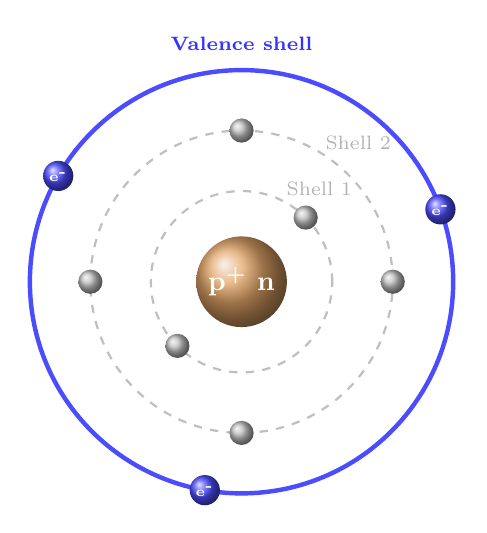
\begin{tikzpicture}[scale=0.48]
            % Núcleo con degradado ocre (solo p+ y n)
            \shade[ball color=orange!80!black!60] (0,0) circle (1.2cm);
            \node[font=\normalsize\bfseries, white] at (0,0) {p\textsuperscript{+} n};
            % Capa 1 (radio 2.4)
            \draw[gray!50, thick, dashed] (0,0) circle (2.4cm);
            % Etiqueta Capa 1: entre capa 1 (2.4) y capa 2 (4.0), a radio ~3.2
            \node[gray!60, font=\scriptsize] at (50:3.2) {Shell 1};
            % Capa 2 (radio 4.0, más separada)
            \draw[gray!50, thick, dashed] (0,0) circle (4.0cm);
            % Etiqueta Capa 2: entre capa 2 (4.0) y valencia (5.6), a radio ~4.8
            \node[gray!60, font=\scriptsize] at (50:4.8) {Shell 2};
            % Capa de valencia (radio 5.6, resaltada)
            \draw[blue!70, ultra thick] (0,0) circle (5.6cm);
            \node[blue!80, font=\scriptsize\bfseries] at (0, 6.3) {Valence shell};
            % Electrones de valencia (azules)
            \foreach \angle in {20, 150, 260} {
                \shade[ball color=blue!70] (\angle:5.6) circle (0.4cm);
                \node[white, font=\tiny\bfseries] at (\angle:5.6) {e\textsuperscript{-}};
            }
            % Electrones internos capa 1 (grises)
            \foreach \angle in {45, 225} {
                \shade[ball color=gray!50] (\angle:2.4) circle (0.32cm);
            }
            % Electrones internos capa 2 (grises)
            \foreach \angle in {0, 90, 180, 270} {
                \shade[ball color=gray!50] (\angle:4.0) circle (0.32cm);
            }
        \end{tikzpicture}
        \caption{Energy levels and valence shell.}
        \label{fig:niveles_capa_de_valencia}
    \end{figure}
\end{minipage}

\subsection{Orbitals: rooms within each floor}
Within each level (each floor), there are different types of "rooms" where electrons can be. These rooms are called \textbf{sublevels} or \textbf{orbitals} and are represented by letters: \textbf{s, p, d, f}
\begin{itemize}
    \item \textbf{Sublevel s}: The simplest, can hold up to \textbf{2 electrons} maximum
    \item \textbf{Sublevel p}: Slightly larger, can hold up to \textbf{6 electrons} maximum
    \item \textbf{Sublevel d}: More spacious, can hold up to \textbf{10 electrons} maximum
    \item \textbf{Sublevel f}: The largest, can hold up to \textbf{14 electrons} maximum
\end{itemize}
\subsection{What orbitals are in each level?}
Not all levels have all types of orbitals. Here is the complete list:
\begin{itemize}
    \item \textbf{Level 1}: only has orbital \textbf{s} → we write \( 1s \)
    \item \textbf{Level 2}: has orbitals \textbf{s} and \textbf{p} → we write \( 2s, 2p \)
    \item \textbf{Level 3}: has \textbf{s, p} and \textbf{d} → we write \( 3s, 3p, 3d \)
    \item \textbf{Level 4}: has \textbf{s, p, d} and \textbf{f} → we write \( 4s, 4p, 4d, 4f \)
    \item \textbf{Levels 5, 6 and 7}: same as level 4, they have s, p, d and f
\end{itemize}
\begin{remark}
    \textbf{Observable pattern:} Each new level adds one more type of orbital. Level 1 only has s, level 2 adds p, level 3 adds d, and level 4 adds f.
\end{remark}
\subsection{How orbitals are written}
When we write an orbital, we use:
\begin{enumerate}
    \item A \textbf{number} indicating the level (1, 2, 3, 4...)
    \item A \textbf{letter} indicating the type of orbital (s, p, d, f)
    \item An \textbf{exponent} (small number above) indicating how many electrons are in that orbital
\end{enumerate}
\textbf{Examples:}
\begin{itemize}
    \item \( 1s^2 \) → In level 1, orbital s, there are 2 electrons
    \item \( 2p^6 \) → In level 2, orbital p, there are 6 electrons
    \item \( 3d^{10} \) → In level 3, orbital d, there are 10 electrons
    \item \( 3s^1 \) → In level 3, orbital s, there is 1 electron
\end{itemize}
\subsection{The Moeller Diagram: the guide for filling orbitals}
Electrons don't fill orbitals in the order we might think (first 1s, then 2s, then 2p...). There is a special order we must follow, and for this we use the \textbf{Moeller Diagram}.
\begin{figure}[H]
    \centering
    \begin{tikzpicture}[>=stealth, font=\sffamily\LARGE\bfseries]

        % --- Configuración de Colores ---
        \definecolor{mygreen}{RGB}{0, 128, 0}
        \definecolor{myblue}{RGB}{91, 155, 213}

        % --- Dibujado de los Subniveles ---
        % Separación horizontal (2.2) y vertical (1.2) para que las diagonales sean perfectas
        \newcommand{\subnivel}[5]{
            \node (n#3#4) at (#1*2.2, -#2*1.2) {#3\textcolor{mygreen}{\textit{#4}}\textsuperscript{\textcolor{red}{#5}}};
        }

        % Columna s (x=0)
        \foreach \n in {1,...,7} \subnivel{0}{\n}{\n}{s}{2};
        % Columna p (x=1)
        \foreach \n in {2,...,7} \subnivel{1}{\n}{\n}{p}{6};
        % Columna d (x=2)
        \foreach \n in {3,...,7} \subnivel{2}{\n}{\n}{d}{10};
        % Columna f (x=3)
        \foreach \n in {4,...,7} \subnivel{3}{\n}{\n}{f}{14};

        % --- Dibujado de las Flechas Diagonales ---
        % Estilo: pasan por el centro, color azul, y se extienden 0.8cm hacia atrás y 1cm hacia adelante
        \tikzset{flecha/.style={myblue, very thick, *->, shorten <=-0.8cm, shorten >=-1cm}}

        % Para flechas que cruzan varios nodos (del centro del primero al centro del último)
        \draw[flecha] ($(n2p.center)+(1.5,0.7)$) -- (n3s.center);
        \draw[flecha] ($(n3p.center)+(1.5,0.7)$) -- (n4s.center);
        \draw[flecha] ($(n3d.center)+(1.5,0.7)$) -- (n5s.center);
        \draw[flecha] ($(n4d.center)+(1.5,0.7)$) -- (n6s.center);
        \draw[flecha] ($(n4f.center)+(1.5,0.7)$) -- (n7s.center);
        \draw[flecha] ($(n5f.center)+(1.5,0.7)$) -- (n7p.center);
        \draw[flecha] ($(n6f.center)+(1.5,0.7)$) -- (n7d.center);

        % Para las flechas de un solo nodo (1s, 2s y 7f), definimos una dirección manual
        % para que mantengan el mismo ángulo que las demás.
        \draw[flecha] ($(n1s.center)+(1.5,0.7)$) -- (n1s.center);
        \draw[flecha] ($(n2s.center)+(1.5,0.7)$) -- (n2s.center);
        \draw[flecha] (n7f.center) ++(1.5,0.8) -- (n7f.center);

    \end{tikzpicture}
    \caption{Moeller Diagram}
    \label{fig:diagrama_moeller}
\end{figure}
\begin{remark}
    \textbf{How to use the Moeller Diagram:} Each arrow tells you which orbitals you should go through. You start with the first arrow (top left) and follow the path of each arrow. The order you get is:
    \[
        1s \rightarrow 2s \rightarrow 2p \rightarrow 3s \rightarrow 3p \rightarrow 4s \rightarrow 3d \rightarrow 4p \rightarrow ...
    \]
\end{remark}
\subsection{How to write an electron configuration step by step}
Let's learn to write the electron configuration of \textbf{Sodium (Na)} which has \( Z = 11 \), that is, 11 electrons.
\begin{enumerate}[label=\textbf{Step \arabic*:}]
        \item \textbf{Identify how many electrons the atom has}

        Sodium has \( Z = 11 \), therefore it has \textbf{11 electrons} that we must place.

        \item \textbf{Follow the Moeller diagram and fill the orbitals in order}

        \begin{itemize}
            \item Arrows are always followed from the starting point to the arrowhead, checking the orbitals we pass through until reaching the arrowhead.

            \item First arrow: In this case it only passes through \( 1s \): This orbital can have a maximum of 2 electrons. We write \( 1s^2 \)

            Electrons placed: 2. We have left: 11 - 2 = 9 electrons.

            \item Second arrow: We have the same situation and it only passes through \( 2s \). This orbital can have a maximum of 2 electrons. We write \( 2s^2 \)

            Electrons placed: 2 (from \( 1s \)) + 2 (from \( 2s \)) = 4. We have left: 11 - 4 = 7 electrons.

            \item Third arrow: now it passes through \( 2p \) and \( 3s \): First we place the electrons in orbital \( 2p \) because it is the first to fill and since we can place a maximum of \num{6} electrons then we write: \( 2p^6 \). Now we have only 1 electron left to place. The next orbital according to the arrow will be \( 3s \), in this case we could put a maximum of \num{2} electrons but since we only have \num{1} electron left to place then we must write: \( 3s^1 \)

            Electrons placed: 2 (from \( 1s \)) + 2 (from \( 2s \)) + 6 (from \( 2p \)) + 1 (from \( 3s \)) = 11. Perfect! We have placed them all

            Electrons placed: 10 + 1 = 11.
        \end{itemize}

        \item \textbf{Write the complete electron configuration}
        \[
            \text{Configuration of Na: } 1s^2\ 2s^2\ 2p^6\ 3s^1
        \]
\end{enumerate}
\begin{remark}
    \textbf{Important tip:} Always count the electrons after each step to make sure you don't exceed the total number of electrons in the atom.
\end{remark}
\begin{example}
    \textbf{Electron configuration of Rubidium (Rb)} with \( Z = 37 \):
    Following the Moeller diagram and counting 37 electrons:
    \[
        1s^2\ 2s^2\ 2p^6\ 3s^2\ 3p^6\ 4s^2\ 3d^{10}\ 4p^6\ 5s^1
    \]

    Note that orbital \( 3d \) fills \textbf{after} \( 4s \), even though 3 is less than 4. This is what the Moeller diagram indicates.
    \textbf{Reordered by levels} (optional, but more organized):
    \[
        1s^2\ 2s^2\ 2p^6\ 3s^2\ 3p^6\ 3d^{10}\ 4s^2\ 4p^6\ 5s^1
    \]
\end{example}
\subsection{Electron configuration of ions}
When an atom becomes an ion (gains or loses electrons), its electron configuration changes:
\begin{itemize}
    \item \textbf{For cations} (positive ions, have lost electrons):

    First write the configuration of the neutral atom, then \textbf{remove electrons from the end} (from the orbital with the highest number).

    \textbf{Example:} \ch{Na^{+}} (has lost 1 electron)
    \begin{itemize}
        \item Neutral Na: \( 1s^2\ 2s^2\ 2p^6\ 3s^1 \)
        \item \ch{Na^{+}}: \( 1s^2\ 2s^2\ 2p^6 \) (we remove 1 electron from \( 3s \))
    \end{itemize}

    \item \textbf{For anions} (negative ions, have gained electrons):
    First write the configuration of the neutral atom, then \textbf{add electrons} following the order of the Moeller diagram.

    \textbf{Example:} \ch{Cl^{-}} (has gained 1 electron)
    \begin{itemize}
        \item Neutral Cl (\( Z = 17 \)): \( 1s^2\ 2s^2\ 2p^6\ 3s^2\ 3p^5 \)
        \item \ch{Cl^{-}}: \( 1s^2\ 2s^2\ 2p^6\ 3s^2\ 3p^6 \) (we add 1 electron to \( 3p \))
    \end{itemize}
\end{itemize}
\begin{exercise}
    Write the electron configuration of Carbon (\( Z = 6 \)) in its ground state (does not lose or gain \el{}).

    \begin{solu}
        \textbf{Given data:}
        \begin{itemize}
            \item Element: Carbon (C)
            \item Atomic number: Z = 6
            \item State: Neutral atom (does not lose or gain electrons)
        \end{itemize}

        \textbf{Step 1:} Determine the number of electrons

        Since the atom is in ground state and is neutral:
        \[
            \text{Number of electrons} = Z = 6
        \]

        \textbf{Step 2:} Remember the orbital filling order

        According to the Aufbau principle, orbitals fill in order of increasing energy:
        \[
            1s \rightarrow 2s \rightarrow 2p \rightarrow 3s \rightarrow 3p \rightarrow 4s \rightarrow 3d \rightarrow \ldots
        \]

        \textbf{Step 3:} Apply the filling rules

        \textbf{Rule 1 - Aufbau Principle:} Fill from the lowest energy orbital.

        \textbf{Rule 2 - Pauli Exclusion Principle:} Each orbital can contain a maximum of 2 electrons with opposite spins.

        \textbf{Rule 3 - Hund's Rule:} In orbitals of equal energy, place one electron in each orbital before pairing.

        \textbf{Step 4:} Distribute the 6 electrons

        \begin{itemize}
            \item \textbf{Orbital 1s:} Holds 2 electrons → \(1s^2\) (4 electrons remaining)
            \item \textbf{Orbital 2s:} Holds 2 electrons → \(2s^2\) (2 electrons remaining)
            \item \textbf{Orbitals 2p:} The remaining 2 electrons go to the 2p orbitals

            Sublevel 2p has 3 orbitals (2p\(_x\), 2p\(_y\), 2p\(_z\)), each can hold 2 electrons (total 6).

            According to Hund's rule, first place one electron in each orbital:
            \[
                2p^2 \quad (\uparrow \quad \uparrow \quad \cdot)
            \]
        \end{itemize}

        \textbf{Step 5:} Write the complete electron configuration
        \[
            \boxed{1s^2 \, 2s^2 \, 2p^2}
        \]

        \textbf{Verification:}
        \[
            2 + 2 + 2 = 6 \text{ electrons} \quad \checkmark
        \]

        \textbf{Answer:} The electron configuration of carbon is: \elconf{C}
    \end{solu}
\end{exercise}
\begin{exercise}
    Determine the electron configuration of Phosphorus (\( Z = 15 \)).
    \begin{solu}
        \textbf{Given data:}
        \begin{itemize}
            \item Element: Phosphorus (P)
            \item Atomic number: Z = 15
            \item State: Neutral atom
        \end{itemize}

        \textbf{Step 1:} Determine the number of electrons
        \[
            \text{Number of electrons} = Z = 15
        \]

        \textbf{Step 2:} Orbital filling order

        For 15 electrons we need:
        \[
            1s \rightarrow 2s \rightarrow 2p \rightarrow 3s \rightarrow 3p
        \]

        \textbf{Step 3:} Distribute the 15 electrons following the rules

        \begin{itemize}
            \item \textbf{Shell n = 1:}
            \begin{itemize}
                \item \(1s^2\) → 2 electrons (13 remaining)
            \end{itemize}

            \item \textbf{Shell n = 2:}
            \begin{itemize}
                \item \(2s^2\) → 2 electrons (11 remaining)
                \item \(2p^6\) → 6 electrons (5 remaining)
            \end{itemize}

            \item \textbf{Shell n = 3:}
            \begin{itemize}
                \item \(3s^2\) → 2 electrons (3 remaining)
                \item \(3p^3\) → 3 electrons (0 remaining)

                The 3 electrons in 3p are distributed according to Hund:
                \[
                    3p^3 \quad (\uparrow \quad \uparrow \quad \uparrow)
                \]
                One electron in each orbital before pairing.
            \end{itemize}
        \end{itemize}

        \textbf{Step 4:} Write the complete electron configuration
        \[
            \boxed{1s^2 \, 2s^2 \, 2p^6 \, 3s^2 \, 3p^3}
        \]

        \textbf{Verification:}
        \[
            2 + 2 + 6 + 2 + 3 = 15 \text{ electrons} \quad \checkmark
        \]

        \textbf{Simplified form (kernel configuration):}

        We can use the previous noble gas (Neon, Z = 10):
        \[
            \text{P:} \quad [\text{Ne}] \, 3s^2 \, 3p^3
        \]

        \textbf{Answer:} The electron configuration of phosphorus is: \elconf{P}
    \end{solu}
\end{exercise}
\begin{exercise}
    Indicate the electron configuration of the chloride anion \ch{Cl^{-}} (\( Z = 17 \)).
    \begin{solu}
        \textbf{Given data:}
        \begin{itemize}
            \item Element: Chlorine (Cl)
            \item Atomic number: Z = 17
            \item Ion: \ch{Cl^{-}} (anion with charge 1-)
        \end{itemize}

        \textbf{Step 1:} Determine the number of electrons in the ion

        The neutral chlorine atom has 17 electrons. Since it is an anion with charge 1-, it has gained 1 electron:
        \[
            \text{Number of electrons} = Z + 1 = 17 + 1 = 18
        \]

        \textbf{Step 2:} Configuration of neutral chlorine atom (17 e\(^-\))

        First we write the configuration of the neutral atom:
        \[
            \text{Cl:} \quad 1s^2 \, 2s^2 \, 2p^6 \, 3s^2 \, 3p^5
        \]

        \textbf{Step 3:} Add the additional electron

        The additional electron is placed in the next available orbital according to the energy order. Since 3p can hold up to 6 electrons and only has 5, the additional electron completes this sublevel:
        \[
            3p^5 + 1e^- \rightarrow 3p^6
        \]

        \textbf{Step 4:} Write the electron configuration of the ion
        \[
            \boxed{\ch{Cl^{-}:} \quad 1s^2 \, 2s^2 \, 2p^6 \, 3s^2 \, 3p^6}
        \]

        \textbf{Verification:}
        \[
            2 + 2 + 6 + 2 + 6 = 18 \text{ electrons} \quad \checkmark
        \]

        \textbf{Important observation:}

        The \ch{Cl^{-}} ion has the same electron configuration as Argon (Ar, Z = 18), a noble gas. We say the chloride ion is isoelectronic with argon:
        \[
            \ch{Cl^{-}:} \quad [\text{Ar}] \quad \text{or} \quad 1s^2 \, 2s^2 \, 2p^6 \, 3s^2 \, 3p^6
        \]

        \textbf{Answer:} The electron configuration of the chloride anion is: \writeelconf{2,2+6,2+6}
    \end{solu}
\end{exercise}
\begin{exercise}
    Write the electron configuration of the oxide ion \ch{O^{2-}} (\( Z = 8 \)).
    \begin{solu}
        \textbf{Given data:}
        \begin{itemize}
            \item Element: Oxygen (O)
            \item Atomic number: Z = 8
            \item Ion: \ch{O^{2-}} (anion with charge 2-)
        \end{itemize}

        \textbf{Step 1:} Determine the number of electrons in the ion

        The neutral oxygen atom has 8 electrons. Since it is an anion with charge 2-, it has gained 2 electrons:
        \[
            \text{Number of electrons} = Z + 2 = 8 + 2 = 10
        \]

        \textbf{Step 2:} Configuration of neutral oxygen atom (8 e\(^-\))

        First we write the configuration of the neutral atom:
        \[
            \text{O:} \quad 1s^2 \, 2s^2 \, 2p^4
        \]

        Electron distribution:
        \begin{itemize}
            \item Shell 1: \(1s^2\) → 2 electrons
            \item Shell 2: \(2s^2\) → 2 electrons
            \item Shell 2: \(2p^4\) → 4 electrons
        \end{itemize}

        \textbf{Step 3:} Add the 2 additional electrons

        The 2 additional electrons are placed in sublevel 2p, which can contain up to 6 electrons:
        \[
            2p^4 + 2e^- \rightarrow 2p^6
        \]

        \textbf{Step 4:} Write the electron configuration of the ion
        \[
            \boxed{\ch{O^{2-}:} \quad 1s^2 \, 2s^2 \, 2p^6}
        \]

        \textbf{Verification:}
        \[
            2 + 2 + 6 = 10 \text{ electrons} \quad \checkmark
        \]

        \textbf{Important observation:}

        The oxide ion \ch{O^{2-}} has the same electron configuration as Neon (Ne, Z = 10), a noble gas. It is isoelectronic with neon and has a very stable configuration:
        \[
            \ch{O^{2-}:} \quad [\text{Ne}] \quad \text{or} \quad 1s^2 \, 2s^2 \, 2p^6
        \]

        This configuration is especially stable because it completes the second electron shell.

        \textbf{Answer:} The electron configuration of the oxide ion is: \writeelconf{2,2+6}
    \end{solu}
\end{exercise}
\begin{exercise}
    Determine the electron configuration of the sulfide anion \ch{S^{2-}} (\( Z = 16 \)).
    \begin{solu}
        \textbf{Given data:}
        \begin{itemize}
            \item Element: Sulfur (S)
            \item Atomic number: Z = 16
            \item Ion: \ch{S^{2-}} (anion with charge 2-)
        \end{itemize}

        \textbf{Step 1:} Determine the number of electrons in the ion

        The neutral sulfur atom has 16 electrons. Since it is an anion with charge 2-, it has gained 2 electrons:
        \[
            \text{Number of electrons} = Z + 2 = 16 + 2 = 18
        \]

        \textbf{Step 2:} Configuration of neutral sulfur atom (16 e\(^-\))

        First we write the configuration of the neutral atom:
        \[
            \text{S:} \quad 1s^2 \, 2s^2 \, 2p^6 \, 3s^2 \, 3p^4
        \]

        Electron distribution:
        \begin{itemize}
            \item Shell 1: \(1s^2\) → 2 electrons
            \item Shell 2: \(2s^2 \, 2p^6\) → 8 electrons
            \item Shell 3: \(3s^2 \, 3p^4\) → 6 electrons
        \end{itemize}

        \textbf{Step 3:} Add the 2 additional electrons

        The 2 additional electrons are placed in sublevel 3p, which can contain up to 6 electrons and currently has 4:
        \[
            3p^4 + 2e^- \rightarrow 3p^6
        \]

        \textbf{Step 4:} Write the electron configuration of the ion
        \[
            \boxed{\ch{S^{2-}:} \quad 1s^2 \, 2s^2 \, 2p^6 \, 3s^2 \, 3p^6}
        \]

        \textbf{Verification:}
        \[
            2 + 2 + 6 + 2 + 6 = 18 \text{ electrons} \quad \checkmark
        \]

        \textbf{Important observation:}

        The sulfide ion \ch{S^{2-}} has the same electron configuration as Argon (Ar, Z = 18), a noble gas. It is isoelectronic with argon:
        \[
            \ch{S^{2-}:} \quad [\text{Ar}] \quad \text{or} \quad 1s^2 \, 2s^2 \, 2p^6 \, 3s^2 \, 3p^6
        \]

        This configuration is very stable because it completes the third shell with 8 electrons (octet rule).

        \textbf{Answer:} The electron configuration of the sulfide anion is: \writeelconf{2,2+6,2+6}
    \end{solu}
\end{exercise}
\begin{exercise}
    Write the electron configuration of the sodium cation \ch{Na^{+}} (\( Z = 11 \)).
    \begin{solu}
        \textbf{Given data:}
        \begin{itemize}
            \item Element: Sodium (Na)
            \item Atomic number: Z = 11
            \item Ion: \ch{Na^{+}} (cation with charge 1+)
        \end{itemize}

        \textbf{Step 1:} Determine the number of electrons in the ion

        The neutral sodium atom has 11 electrons. Since it is a cation with charge 1+, it has lost 1 electron:
        \[
            \text{Number of electrons} = Z - 1 = 11 - 1 = 10
        \]

        \textbf{Step 2:} Configuration of neutral sodium atom (11 e\(^-\))

        First we write the configuration of the neutral atom:
        \[
            \text{Na:} \quad 1s^2 \, 2s^2 \, 2p^6 \, 3s^1
        \]

        Electron distribution:
        \begin{itemize}
            \item Shell 1: \(1s^2\) → 2 electrons
            \item Shell 2: \(2s^2 \, 2p^6\) → 8 electrons
            \item Shell 3: \(3s^1\) → 1 electron
        \end{itemize}

        \textbf{Step 3:} Remove the lost electron

        When an atom loses electrons, it loses them from the outermost shell (highest energy level). Sodium loses its only electron from shell 3:
        \[
            3s^1 - 1e^- \rightarrow 3s^0 \quad \text{(removed)}
        \]

        \textbf{Step 4:} Write the electron configuration of the ion
        \[
            \boxed{\ch{Na^{+}:} \quad 1s^2 \, 2s^2 \, 2p^6}
        \]

        \textbf{Verification:}
        \[
            2 + 2 + 6 = 10 \text{ electrons} \quad \checkmark
        \]

        \textbf{Important observation:}

        The \ch{Na^{+}} cation has the same electron configuration as Neon (Ne, Z = 10), a noble gas. It is isoelectronic with neon:
        \[
            \ch{Na^{+}:} \quad [\text{Ne}] \quad \text{or} \quad 1s^2 \, 2s^2 \, 2p^6
        \]

        By losing its valence electron (\(3s^1\)), sodium achieves the stable noble gas configuration, which is why it tends to form the \ch{Na^{+}} cation easily.

        \textbf{Answer:} The electron configuration of the sodium cation is: \writeelconf{2,2+6}
    \end{solu}
\end{exercise}
\begin{exercise}
    Indicate the electron configuration of the calcium ion \ch{Ca^{2+}} (\( Z = 20 \)).
    \begin{solu}
        \textbf{Given data:}
        \begin{itemize}
            \item Element: Calcium (Ca)
            \item Atomic number: Z = 20
            \item Ion: \ch{Ca^{2+}} (cation with charge 2+)
        \end{itemize}

        \textbf{Step 1:} Determine the number of electrons in the ion

        The neutral calcium atom has 20 electrons. Since it is a cation with charge 2+, it has lost 2 electrons:
        \[
            \text{Number of electrons} = Z - 2 = 20 - 2 = 18
        \]

        \textbf{Step 2:} Configuration of neutral calcium atom (20 e\(^-\))

        First we write the configuration of the neutral atom:
        \[
            \text{Ca:} \quad 1s^2 \, 2s^2 \, 2p^6 \, 3s^2 \, 3p^6 \, 4s^2
        \]

        Electron distribution:
        \begin{itemize}
            \item Shell 1: \(1s^2\) → 2 electrons
            \item Shell 2: \(2s^2 \, 2p^6\) → 8 electrons
            \item Shell 3: \(3s^2 \, 3p^6\) → 8 electrons
            \item Shell 4: \(4s^2\) → 2 electrons
        \end{itemize}

        \textbf{Step 3:} Remove the 2 lost electrons

        Electrons are lost from the outermost shell (highest energy level). Calcium loses its 2 electrons from shell 4:
        \[
            4s^2 - 2e^- \rightarrow 4s^0 \quad \text{(removed)}
        \]

        \textbf{Step 4:} Write the electron configuration of the ion
        \[
            \boxed{\ch{Ca^{2+}:} \quad 1s^2 \, 2s^2 \, 2p^6 \, 3s^2 \, 3p^6}
        \]

        \textbf{Verification:}
        \[
            2 + 2 + 6 + 2 + 6 = 18 \text{ electrons} \quad \checkmark
        \]

        \textbf{Important observation:}

        The \ch{Ca^{2+}} cation has the same electron configuration as Argon (Ar, Z = 18), a noble gas. It is isoelectronic with argon:
        \[
            \ch{Ca^{2+}:} \quad [\text{Ar}] \quad \text{or} \quad 1s^2 \, 2s^2 \, 2p^6 \, 3s^2 \, 3p^6
        \]

        By losing its 2 valence electrons (\(4s^2\)), calcium achieves the stable noble gas configuration with 8 electrons in its outermost shell (octet rule), which is why it tends to form the \ch{Ca^{2+}} cation easily.

        \textbf{Answer:} The electron configuration of the calcium ion is: \writeelconf{2,2+6,2+6}
    \end{solu}
\end{exercise}
\subsection{Valence shell and valence electrons}
The outermost shell or level of an atom is very important because it determines how that atom will behave chemically.
\begin{definition}{Valence Shell}
    The \textbf{valence shell} is the highest energy level (the largest number) that has electrons. It is the outermost shell of the atom.
\end{definition}
\begin{definition}{Valence electrons}
    \textbf{Valence electrons} are all the electrons that are in the valence shell. They are the outermost electrons and are the ones that participate in chemical reactions.
\end{definition}
\begin{remark}
    \textbf{Why are valence electrons important?} They are like the atom's ``hands'': with them it can form chemical bonds with other atoms. Inner electrons are too close to the nucleus and do not participate in reactions.
\end{remark}
\begin{example}
    \textbf{Sodium (Na):} \( 1s^2\ 2s^2\ 2p^6\ 3s^1 \)
    \begin{itemize}
        \item Valence shell: \textbf{n = 3} (the highest number that appears)
        \item Valence electrons: \textbf{1 electron} (the one in \( 3s^1 \))
    \end{itemize}

    \textbf{Oxygen (O):} \( 1s^2\ 2s^2\ 2p^4 \)
    \begin{itemize}
        \item Valence shell: \textbf{n = 2}
        \item Valence electrons: \textbf{6 electrons} (2 in \( 2s \) + 4 in \( 2p \) = 6)
    \end{itemize}

    \textbf{Carbon (C):} \( 1s^2\ 2s^2\ 2p^2 \)
    \begin{itemize}
        \item Valence shell: \textbf{n = 2}
        \item Valence electrons: \textbf{4 electrons} (2 in \( 2s \) + 2 in \( 2p \) = 4)
    \end{itemize}
\end{example}
\begin{remark}
    \textbf{Connection with the periodic table:} Elements in the same group (same column) have the same number of valence electrons. That's why they have similar chemical properties. We'll see this in the next section!
\end{remark}
\begin{exercise}
    Identify the valence shell and the number of valence electrons of Lithium (\( Z = 3 \)).
    \begin{solu}
        \textbf{Given data:}
        \begin{itemize}
            \item Element: Lithium (Li)
            \item Atomic number: Z = 3
            \item State: Neutral atom
        \end{itemize}

        \textbf{Step 1:} Determine the number of electrons
        \[
            \text{Number of electrons} = Z = 3
        \]

        \textbf{Step 2:} Write the electron configuration

        We distribute the 3 electrons following the filling order:
        \begin{itemize}
            \item Orbital \(1s\): 2 electrons → \(1s^2\)
            \item Orbital \(2s\): 1 electron → \(2s^1\)
        \end{itemize}

        Complete electron configuration:
        \[
            \text{Li:} \quad 1s^2 \, 2s^1
        \]

        \textbf{Verification:}
        \[
            2 + 1 = 3 \text{ electrons} \quad \checkmark
        \]

        \textbf{Step 3:} Identify the valence shell

        The valence shell is the outermost shell (with the highest principal quantum number \(n\)).

        Analyzing the configuration:
        \begin{itemize}
            \item Shell 1 (\(n = 1\)): \(1s^2\) → complete shell (inner)
            \item Shell 2 (\(n = 2\)): \(2s^1\) → outermost shell
        \end{itemize}

        Therefore, the valence shell is:
        \[
            \boxed{n = 2}
        \]

        \textbf{Step 4:} Count the valence electrons

        Valence electrons are those found in the outermost shell:
        \[
            \text{Electrons in shell } n = 2: \quad 2s^1 \rightarrow 1 \text{ electron}
        \]

        Therefore:
        \[
            \boxed{\text{Valence electrons} = 1}
        \]

        \textbf{Answer:}
        \begin{itemize}
            \item Electron configuration: \elconf{Li}
            \item Valence shell: \(n = 2\)
            \item Valence electrons: 1
        \end{itemize}
    \end{solu}
\end{exercise}
\begin{exercise}
    Determine the valence shell and valence electrons of Nitrogen (\( Z = 7 \)).
    \begin{solu}
        \textbf{Given data:}
        \begin{itemize}
            \item Element: Nitrogen (N)
            \item Atomic number: Z = 7
            \item State: Neutral atom
        \end{itemize}

        \textbf{Step 1:} Determine the number of electrons
        \[
            \text{Number of electrons} = Z = 7
        \]

        \textbf{Step 2:} Write the electron configuration

        We distribute the 7 electrons following the filling order:
        \begin{itemize}
            \item Shell 1 (\(n = 1\)):
            \begin{itemize}
                \item \(1s^2\) → 2 electrons
            \end{itemize}
            \item Shell 2 (\(n = 2\)):
            \begin{itemize}
                \item \(2s^2\) → 2 electrons
                \item \(2p^3\) → 3 electrons
            \end{itemize}
        \end{itemize}

        Complete electron configuration:
        \[
            \text{N:} \quad 1s^2 \, 2s^2 \, 2p^3
        \]

        \textbf{Verification:}
        \[
            2 + 2 + 3 = 7 \text{ electrons} \quad \checkmark
        \]

        \textbf{Step 3:} Identify the valence shell

        The valence shell is the outermost shell.

        Analyzing the configuration:
        \begin{itemize}
            \item Shell 1 (\(n = 1\)): \(1s^2\) → complete shell (inner)
            \item Shell 2 (\(n = 2\)): \(2s^2 \, 2p^3\) → outermost shell
        \end{itemize}

        Therefore, the valence shell is:
        \[
            \boxed{n = 2}
        \]

        \textbf{Step 4:} Count the valence electrons

        Valence electrons are all electrons in the outermost shell:
        \[
            \text{Electrons in shell } n = 2: \quad 2s^2 + 2p^3 = 2 + 3 = 5 \text{ electrons}
        \]

        Therefore:
        \[
            \boxed{\text{Valence electrons} = 5}
        \]

        \textbf{Observation:}

        Nitrogen has 5 valence electrons, which means it needs 3 electrons to complete its valence shell (octet rule). That's why it tends to form 3 covalent bonds.

        \textbf{Answer:}
        \begin{itemize}
            \item Electron configuration: \elconf{N}
            \item Valence shell: \(n = 2\)
            \item Valence electrons: 5
        \end{itemize}
    \end{solu}
\end{exercise}
\begin{exercise}
    For the Magnesium atom (\( Z = 12 \)), indicate its configuration and valence electrons.
    \begin{solu}
        \textbf{Given data:}
        \begin{itemize}
            \item Element: Magnesium (Mg)
            \item Atomic number: Z = 12
            \item State: Neutral atom
        \end{itemize}

        \textbf{Step 1:} Determine the number of electrons
        \[
            \text{Number of electrons} = Z = 12
        \]

        \textbf{Step 2:} Write the electron configuration

        We distribute the 12 electrons following the filling order:
        \begin{itemize}
            \item Shell 1 (\(n = 1\)):
            \begin{itemize}
                \item \(1s^2\) → 2 electrons (10 remaining)
            \end{itemize}
            \item Shell 2 (\(n = 2\)):
            \begin{itemize}
                \item \(2s^2\) → 2 electrons (8 remaining)
                \item \(2p^6\) → 6 electrons (2 remaining)
            \end{itemize}
            \item Shell 3 (\(n = 3\)):
            \begin{itemize}
                \item \(3s^2\) → 2 electrons (0 remaining)
            \end{itemize}
        \end{itemize}

        Complete electron configuration:
        \[
            \text{Mg:} \quad 1s^2 \, 2s^2 \, 2p^6 \, 3s^2
        \]

        \textbf{Verification:}
        \[
            2 + 2 + 6 + 2 = 12 \text{ electrons} \quad \checkmark
        \]

        \textbf{Simplified form:}

        Using the previous noble gas (Neon, Z = 10):
        \[
            \text{Mg:} \quad [\text{Ne}] \, 3s^2
        \]

        \textbf{Step 3:} Identify the valence shell

        The valence shell is the outermost shell.

        Analyzing the configuration:
        \begin{itemize}
            \item Shells 1 and 2 (\(n = 1, 2\)): complete (inner)
            \item Shell 3 (\(n = 3\)): \(3s^2\) → outermost shell
        \end{itemize}

        Therefore, the valence shell is:
        \[
            \boxed{n = 3}
        \]

        \textbf{Step 4:} Count the valence electrons

        Valence electrons are the electrons in the outermost shell:
        \[
            \text{Electrons in shell } n = 3: \quad 3s^2 = 2 \text{ electrons}
        \]

        Therefore:
        \[
            \boxed{\text{Valence electrons} = 2}
        \]

        \textbf{Observation:}

        Magnesium has 2 valence electrons, so it tends to lose these 2 electrons to form the \ch{Mg^{2+}} ion and achieve the stable neon configuration.

        \textbf{Answer:}
        \begin{itemize}
            \item Electron configuration: \elconf{Mg}
            \item Valence shell: \(n = 3\)
            \item Valence electrons: 2
        \end{itemize}
    \end{solu}
\end{exercise}
\begin{exercise}
    Write the configuration of Aluminum (\( Z = 13 \)) and identify its valence shell.
    \begin{solu}
        \textbf{Given data:}
        \begin{itemize}
            \item Element: Aluminum (Al)
            \item Atomic number: Z = 13
            \item State: Neutral atom
        \end{itemize}

        \textbf{Step 1:} Determine the number of electrons
        \[
            \text{Number of electrons} = Z = 13
        \]

        \textbf{Step 2:} Write the electron configuration

        We distribute the 13 electrons following the filling order:
        \begin{itemize}
            \item Shell 1 (\(n = 1\)):
            \begin{itemize}
                \item \(1s^2\) → 2 electrons (11 remaining)
            \end{itemize}
            \item Shell 2 (\(n = 2\)):
            \begin{itemize}
                \item \(2s^2\) → 2 electrons (9 remaining)
                \item \(2p^6\) → 6 electrons (3 remaining)
            \end{itemize}
            \item Shell 3 (\(n = 3\)):
            \begin{itemize}
                \item \(3s^2\) → 2 electrons (1 remaining)
                \item \(3p^1\) → 1 electron (0 remaining)
            \end{itemize}
        \end{itemize}

        Complete electron configuration:
        \[
            \text{Al:} \quad 1s^2 \, 2s^2 \, 2p^6 \, 3s^2 \, 3p^1
        \]

        \textbf{Verification:}
        \[
            2 + 2 + 6 + 2 + 1 = 13 \text{ electrons} \quad \checkmark
        \]

        \textbf{Simplified form:}

        Using the previous noble gas (Neon, Z = 10):
        \[
            \text{Al:} \quad [\text{Ne}] \, 3s^2 \, 3p^1
        \]

        \textbf{Step 3:} Identify the valence shell

        The valence shell is the outermost shell.

        Analyzing the configuration:
        \begin{itemize}
            \item Shells 1 and 2 (\(n = 1, 2\)): complete (inner)
            \item Shell 3 (\(n = 3\)): \(3s^2 \, 3p^1\) → outermost shell
        \end{itemize}

        Therefore, the valence shell is:
        \[
            \boxed{n = 3}
        \]

        \textbf{Step 4:} Count the valence electrons

        Valence electrons are all electrons in the outermost shell:
        \[
            \text{Electrons in shell } n = 3: \quad 3s^2 + 3p^1 = 2 + 1 = 3 \text{ electrons}
        \]

        Therefore:
        \[
            \boxed{\text{Valence electrons} = 3}
        \]

        \textbf{Observation:}

        Aluminum has 3 valence electrons, so it tends to lose these 3 electrons to form the \ch{Al^{3+}} ion and achieve the stable neon configuration. It can also form 3 covalent bonds.

        \textbf{Answer:}
        \begin{itemize}
            \item Electron configuration: \elconf{Al}
            \item Valence shell: \(n = 3\)
            \item Valence electrons: 3
        \end{itemize}
    \end{solu}
\end{exercise}
\begin{exercise}
    Determine the valence electrons of Sulfur (\( Z = 16 \)).
    \begin{solu}
        \textbf{Given data:}
        \begin{itemize}
            \item Element: Sulfur (S)
            \item Atomic number: Z = 16
            \item State: Neutral atom
        \end{itemize}

        \textbf{Step 1:} Determine the number of electrons
        \[
            \text{Number of electrons} = Z = 16
        \]

        \textbf{Step 2:} Write the electron configuration

        We distribute the 16 electrons following the filling order:
        \begin{itemize}
            \item Shell 1 (\(n = 1\)):
            \begin{itemize}
                \item \(1s^2\) → 2 electrons (14 remaining)
            \end{itemize}
            \item Shell 2 (\(n = 2\)):
            \begin{itemize}
                \item \(2s^2\) → 2 electrons (12 remaining)
                \item \(2p^6\) → 6 electrons (6 remaining)
            \end{itemize}
            \item Shell 3 (\(n = 3\)):
            \begin{itemize}
                \item \(3s^2\) → 2 electrons (4 remaining)
                \item \(3p^4\) → 4 electrons (0 remaining)
            \end{itemize}
        \end{itemize}

        Complete electron configuration:
        \[
            \text{S:} \quad 1s^2 \, 2s^2 \, 2p^6 \, 3s^2 \, 3p^4
        \]

        \textbf{Verification:}
        \[
            2 + 2 + 6 + 2 + 4 = 16 \text{ electrons} \quad \checkmark
        \]

        \textbf{Simplified form:}

        Using the previous noble gas (Neon, Z = 10):
        \[
            \text{S:} \quad [\text{Ne}] \, 3s^2 \, 3p^4
        \]

        \textbf{Step 3:} Identify the valence shell

        The valence shell is the outermost shell.

        Analyzing the configuration:
        \begin{itemize}
            \item Shells 1 and 2 (\(n = 1, 2\)): complete (inner)
            \item Shell 3 (\(n = 3\)): \(3s^2 \, 3p^4\) → outermost shell
        \end{itemize}

        Therefore, the valence shell is:
        \[
            \boxed{n = 3}
        \]

        \textbf{Step 4:} Count the valence electrons

        Valence electrons are all electrons in the outermost shell:
        \[
            \text{Electrons in shell } n = 3: \quad 3s^2 + 3p^4 = 2 + 4 = 6 \text{ electrons}
        \]

        Therefore:
        \[
            \boxed{\text{Valence electrons} = 6}
        \]

        \textbf{Observation:}

        Sulfur has 6 valence electrons, which means it needs 2 electrons to complete its valence shell (octet rule). That's why it tends to:
        \begin{itemize}
            \item Gain 2 electrons to form the \ch{S^{2-}} ion (isoelectronic with Ar)
            \item Form 2 covalent bonds (as in \ch{H2S})
        \end{itemize}

        \textbf{Answer:}
        \begin{itemize}
            \item Electron configuration: \elconf{S}
            \item Valence shell: \(n = 3\)
            \item Valence electrons: 6
        \end{itemize}
    \end{solu}
\end{exercise}
\section{The Periodic System of Elements}
The Periodic System, also called the Periodic Table, is a fundamental tool in chemistry that organizes all known chemical elements.
\subsection{History and Organization}
It was created by the Russian chemist \textbf{Dmitri Mendeleev} in 1869. Mendeleev organized the elements in order of increasing atomic mass and observed that chemical properties repeated periodically.
\begin{remark}
    \textbf{Interesting fact:} Mendeleev left gaps in his table for elements that had not yet been discovered. He even predicted their properties! Years later, when those elements were discovered, their properties matched Mendeleev's predictions.
\end{remark}
In the current periodic table, elements are arranged in \textbf{increasing atomic number} (from lowest to highest \( Z \)) and organized into:
\begin{itemize}
    \item \negsubro{Horizontal rows} called \textbf{periods}. There are 7 periods numbered from 1 to 7.
    \item \negsubro{Vertical columns} called \textbf{groups} or \textbf{families}. There are 18 groups numbered from 1 to 18.
\end{itemize}

\subsection{Periods}
\textbf{Periods} are the horizontal rows of the periodic table. The period number indicates how many electron shells an atom of that element has.
\begin{itemize}
    \item Period 1: elements with 1 electron shell (H, He)
    \item Period 2: elements with 2 electron shells (Li, Be, B, C, N, O, F, Ne)
    \item Period 3: elements with 3 electron shells (Na, Mg, Al, Si, P, S, Cl, Ar)
    \item And so on...
\end{itemize}

\subsection{Groups or Families}
\textbf{Groups} are the vertical columns. Elements in the same group have similar chemical properties because they have the same number of electrons in their outermost shell.
Some groups have special names due to their characteristic properties:
\begin{itemize}
    \item \textbf{Group 1 - Alkali metals}: They are very reactive metals (Li, Na, K, Rb, Cs, Fr). They react violently with water.
    \item \textbf{Group 2 - Alkaline earth metals}: They are less reactive metals than alkali metals (Be, Mg, Ca, Sr, Ba, Ra).
    \item \textbf{Groups 3 to 12 - Transition metals}: They include many well-known metals such as iron (Fe), copper (Cu), silver (Ag), gold (Au), etc.
    \item \textbf{Group 13 - Boron group}: Notable members include boron (B) and aluminum (Al).
    \item \textbf{Group 14 - Carbon group}: Includes carbon (C), silicon (Si), etc.
    \item \textbf{Group 15 - Nitrogen group}: Includes nitrogen (N) and phosphorus (P).
    \item \textbf{Group 16 - Chalcogens}: Includes oxygen (O) and sulfur (S).
    \item \textbf{Group 17 - Halogens}: They are very reactive nonmetals (F, Cl, Br, I, At). Chlorine is used to disinfect swimming pool water.
    \item \textbf{Group 18 - Noble gases}: They are gases that hardly react with anything (He, Ne, Ar, Kr, Xe, Rn). Helium is used to inflate balloons.
\end{itemize}
\begin{remark}
    \textbf{Memory trick:} Elements in the same group (same column) resemble each other, like siblings in a family. That's why they are called ``families''.
\end{remark}
\subsection{Metals, Nonmetals, and Metalloids}
Elements are also classified according to their properties into:
\begin{itemize}
    \item \negsubro{Metals}: Shiny, good conductors of heat and electricity, malleable and ductile. Most elements are metals. Examples: Fe, Cu, Au, Ag, Al.
    \item \negsubro{Nonmetals}: Not shiny, poor conductors, brittle. They are on the right side of the table. Examples: O, N, C, S, Cl.
    \item \negsubro{Metalloids}: They have intermediate properties. They are used in electronics. Examples: Si, Ge, As.
\end{itemize}
\begin{exercise}
    Indicate the group and period in which the following elements are found: nitrogen, aluminum, krypton, silver, rubidium, titanium, cesium, and lead.
    \begin{solu}
        To locate each element in the periodic table, we need to identify:
        \begin{itemize}
            \item \textbf{Period:} Horizontal row in which the element is found (indicates the number of electron shells)
            \item \textbf{Group:} Vertical column in which the element is found (indicates the number of valence electrons for representative elements)
        \end{itemize}

        \textbf{Method:} We locate each element in the periodic table and note its position.

        \textbf{1. Nitrogen (N, Z = 7)}

        \textbf{Step 1:} Electron configuration: \(1s^2 \, 2s^2 \, 2p^3\)

        \textbf{Step 2:} Identify period and group
        \begin{itemize}
            \item The outermost shell is \(n = 2\) → \textbf{Period 2}
            \item Valence electrons: 5 (\(2s^2 \, 2p^3\)) → \textbf{Group 15}
        \end{itemize}

        \textbf{Answer:} Group 15, Period 2

        \textbf{2. Aluminum (Al, Z = 13)}

        \textbf{Step 1:} Electron configuration: \(1s^2 \, 2s^2 \, 2p^6 \, 3s^2 \, 3p^1\)

        \textbf{Step 2:} Identify period and group
        \begin{itemize}
            \item The outermost shell is \(n = 3\) → \textbf{Period 3}
            \item Valence electrons: 3 (\(3s^2 \, 3p^1\)) → \textbf{Group 13}
        \end{itemize}

        \textbf{Answer:} Group 13, Period 3

        \textbf{3. Krypton (Kr, Z = 36)}

        \textbf{Step 1:} Electron configuration: \([\text{Ar}] \, 3d^{10} \, 4s^2 \, 4p^6\)

        \textbf{Step 2:} Identify period and group
        \begin{itemize}
            \item The outermost shell is \(n = 4\) → \textbf{Period 4}
            \item Noble gas with 8 valence electrons → \textbf{Group 18}
        \end{itemize}

        \textbf{Answer:} Group 18, Period 4

        \textbf{4. Silver (Ag, Z = 47)}

        \textbf{Step 1:} Silver is a transition metal

        \textbf{Step 2:} Identify period and group
        \begin{itemize}
            \item Location in the table: → \textbf{Period 5}
            \item Transition metal → \textbf{Group 11}
        \end{itemize}

        \textbf{Answer:} Group 11, Period 5

        \textbf{5. Rubidium (Rb, Z = 37)}

        \textbf{Step 1:} Electron configuration: \([\text{Kr}] \, 5s^1\)

        \textbf{Step 2:} Identify period and group
        \begin{itemize}
            \item The outermost shell is \(n = 5\) → \textbf{Period 5}
            \item 1 valence electron, alkali metal → \textbf{Group 1}
        \end{itemize}

        \textbf{Answer:} Group 1, Period 5

        \textbf{6. Titanium (Ti, Z = 22)}

        \textbf{Step 1:} Electron configuration: \([\text{Ar}] \, 3d^2 \, 4s^2\)

        \textbf{Step 2:} Identify period and group
        \begin{itemize}
            \item The outermost shell is \(n = 4\) → \textbf{Period 4}
            \item Transition metal → \textbf{Group 4}
        \end{itemize}

        \textbf{Answer:} Group 4, Period 4

        \textbf{7. Cesium (Cs, Z = 55)}

        \textbf{Step 1:} Electron configuration: \([\text{Xe}] \, 6s^1\)

        \textbf{Step 2:} Identify period and group
        \begin{itemize}
            \item The outermost shell is \(n = 6\) → \textbf{Period 6}
            \item 1 valence electron, alkali metal → \textbf{Group 1}
        \end{itemize}

        \textbf{Answer:} Group 1, Period 6

        \textbf{8. Lead (Pb, Z = 82)}

        \textbf{Step 1:} Electron configuration: \([\text{Xe}] \, 4f^{14} \, 5d^{10} \, 6s^2 \, 6p^2\)

        \textbf{Step 2:} Identify period and group
        \begin{itemize}
            \item The outermost shell is \(n = 6\) → \textbf{Period 6}
            \item 4 valence electrons (\(6s^2 \, 6p^2\)) → \textbf{Group 14}
        \end{itemize}

        \textbf{Answer:} Group 14, Period 6

        \textbf{Summary of answers:}
        \begin{center}
            % --- tabla antigua ---
            % \begin{tabular}{|l|c|c|}
                % \hline
                % \textbf{Element} & \textbf{Group} & \textbf{Period} \\
                % \hline
                % Nitrogen (N)     & 15             & 2               \\
                % \hline
                % Aluminum (Al)    & 13             & 3               \\
                % \hline
                % Krypton (Kr)     & 18             & 4               \\
                % \hline
                % Silver (Ag)      & 11             & 5               \\
                % \hline
                % Rubidium (Rb)    & 1              & 5               \\
                % \hline
                % Titanium (Ti)    & 4              & 4               \\
                % \hline
                % Cesium (Cs)      & 1              & 6               \\
                % \hline
                % Lead (Pb)        & 14             & 6               \\
                % \hline
            % \end{tabular}
            % --- tabla nueva ---
            \begin{tabular}{@{}lcc@{}}
                \toprule
                \textbf{Element} & \textbf{Group} & \textbf{Period} \\
                \midrule
                Nitrogen (N) & 15 & 2 \\[3pt]
                Aluminum (Al) & 13 & 3 \\[3pt]
                Krypton (Kr) & 18 & 4 \\[3pt]
                Silver (Ag) & 11 & 5 \\[3pt]
                Rubidium (Rb) & 1 & 5 \\[3pt]
                Titanium (Ti) & 4 & 4 \\[3pt]
                Cesium (Cs) & 1 & 6 \\[3pt]
                Lead (Pb) & 14 & 6 \\
                \bottomrule
            \end{tabular}
        \end{center}
    \end{solu}
\end{exercise}
\begin{exercise}
    Write the symbol of the following elements:
    \begin{multicols}{4}
        \begin{enumerate}[label=\letraminuscula]
        \item magnesium
        \item carbon
        \item aluminum
        \item argon
        \item lithium
        \item silicon
        \item copper
        \item zinc
        \item helium
        \item phosphorus
        \item palladium
        \item rubidium
        \end{enumerate}
    \end{multicols}
    \begin{solu}
        To write the chemical symbol of each element, we must remember that:
        \begin{itemize}
            \item Chemical symbols consist of one or two letters
            \item The first letter is always uppercase
            \item The second letter (if it exists) is always lowercase
            \item Symbols come from the Latin name or common name of the element
        \end{itemize}

        \textbf{Detailed solution:}

        \textbf{a) Magnesium}

        Symbol: \textbf{Mg}

        Explanation: From Latin "Magnesium". First letter M (uppercase) + second letter g (lowercase).

        \textbf{b) Carbon}

        Symbol: \textbf{C}

        Explanation: From Latin "Carbonium". Only one uppercase letter.

        \textbf{c) Aluminum}

        Symbol: \textbf{Al}

        Explanation: From Latin "Aluminium". First letter A (uppercase) + second letter l (lowercase).

        \textbf{d) Argon}

        Symbol: \textbf{Ar}

        Explanation: From Greek "Argon". First letter A (uppercase) + second letter r (lowercase).

        \textbf{e) Lithium}

        Symbol: \textbf{Li}

        Explanation: From Greek "Lithion". First letter L (uppercase) + second letter i (lowercase).

        \textbf{f) Silicon}

        Symbol: \textbf{Si}

        Explanation: From Latin "Silicium". First letter S (uppercase) + second letter i (lowercase).

        \textbf{g) Copper}

        Symbol: \textbf{Cu}

        Explanation: From Latin "Cuprum". First letter C (uppercase) + second letter u (lowercase).

        \textbf{h) Zinc}

        Symbol: \textbf{Zn}

        Explanation: From German "Zink". First letter Z (uppercase) + second letter n (lowercase).

        \textbf{i) Helium}

        Symbol: \textbf{He}

        Explanation: From Greek "Helios" (sun). First letter H (uppercase) + second letter e (lowercase).

        \textbf{j) Phosphorus}

        Symbol: \textbf{P}

        Explanation: From Greek "Phosphoros". Only one uppercase letter.

        \textbf{k) Palladium}

        Symbol: \textbf{Pd}

        Explanation: From asteroid Pallas. First letter P (uppercase) + second letter d (lowercase).

        \textbf{l) Rubidium}

        Symbol: \textbf{Rb}

        Explanation: From Latin "Rubidus" (red). First letter R (uppercase) + second letter b (lowercase).

        \textbf{Summary of answers:}
        \begin{multicols}{3}
            \begin{enumerate}[label=\letraminuscula]
                \item Mg
                \item C
                \item Al
                \item Ar
                \item Li
                \item Si
                \item Cu
                \item Zn
                \item He
                \item P
                \item Pd
                \item Rb
            \end{enumerate}
        \end{multicols}
    \end{solu}
\end{exercise}

\begin{exercise}
    Write the name of the following elements:
    \begin{multicols}{4}
        \begin{enumerate}[label=\letraminuscula]
        \item O
        \item N
        \item Ni
        \item H
        \item Ne
        \item Mn
        \item Ag
        \item Au
        \item Hg
        \item I
        \item Cu
        \item Pt
        \end{enumerate}
    \end{multicols}
    \begin{solu}
        To identify the name of each element from its chemical symbol, we must know the periodic table. Some symbols come from the Latin name of the element.

        \textbf{Detailed solution:}

        \textbf{a) O}

        Name: \textbf{Oxygen}

        Explanation: Z = 8. Nonmetal from group 16 (chalcogens). From Greek "oxys" (acid) and "genes" (generator). Essential for respiration.

        \textbf{b) N}

        Name: \textbf{Nitrogen}

        Explanation: Z = 7. Nonmetal from group 15. From Greek "nitron" (saltpeter) and "genes" (generator). Main component of air (\(\sim\)78\%).

        \textbf{c) Ni}

        Name: \textbf{Nickel}

        Explanation: Z = 28. Transition metal from group 10. From German "kupfernickel" (devil's copper). Metal used in coins and alloys.

        \textbf{d) H}

        Name: \textbf{Hydrogen}

        Explanation: Z = 1. Nonmetal from group 1. From Greek "hydro" (water) and "genes" (generator). The most abundant element in the universe.

        \textbf{e) Ne}

        Name: \textbf{Neon}

        Explanation: Z = 10. Noble gas from group 18. From Greek "neos" (new). Used in neon lights for its characteristic glow.

        \textbf{f) Mn}

        Name: \textbf{Manganese}

        Explanation: Z = 25. Transition metal from group 7. From Latin "magnes" (magnet). Important in steel production.

        \textbf{g) Ag}

        Name: \textbf{Silver}

        Explanation: Z = 47. Transition metal from group 11. From Latin "Argentum". Precious metal with the highest electrical conductivity.

        \textbf{h) Au}

        Name: \textbf{Gold}

        Explanation: Z = 79. Transition metal from group 11. From Latin "Aurum". Highly valued precious metal, very ductile and malleable.

        \textbf{i) Hg}

        Name: \textbf{Mercury}

        Explanation: Z = 80. Transition metal from group 12. From Latin "Hydrargyrum" (liquid silver). The only metal that is liquid at room temperature.

        \textbf{j) I}

        Name: \textbf{Iodine}

        Explanation: Z = 53. Halogen from group 17. From Greek "iodes" (violet). Essential for thyroid function.

        \textbf{k) Cu}

        Name: \textbf{Copper}

        Explanation: Z = 29. Transition metal from group 11. From Latin "Cuprum" (from Cyprus). Excellent electrical conductor, characteristic reddish color.

        \textbf{l) Pt}

        Name: \textbf{Platinum}

        Explanation: Z = 78. Transition metal from group 10. From Spanish "platina" (little silver). Precious metal very resistant to corrosion.

        \textbf{Summary of answers:}
        \begin{multicols}{3}
            \begin{enumerate}[label=\letraminuscula]
                \item Oxygen
                \item Nitrogen
                \item Nickel
                \item Hydrogen
                \item Neon
                \item Manganese
                \item Silver
                \item Gold
                \item Mercury
                \item Iodine
                \item Copper
                \item Platinum
            \end{enumerate}
        \end{multicols}
    \end{solu}
\end{exercise}

\begin{exercise}
    Write the name and symbol of the following elements given their group and period.
    \begin{multicols}{3}
        \begin{enumerate}[label=\letraminuscula]
        \item Group 1 Period 4
        \item Group 18 Period 2
        \item Group 13 Period 3
        \item Group 2 Period 5
        \item Group 14 Period 4
        \item Group 12 Period 5
        \item Group 10 Period 4
        \item Group 16 Period 2
        \item Group 15 Period 5
        \item Group 14 Period 3
        \item Group 18 Period 6
        \item Group 8 Period 4
        \end{enumerate}
    \end{multicols}
    \begin{solu}
        To identify each element, we must locate it in the periodic table using the coordinates of group (column) and period (row).

        \textbf{Method:}
        \begin{enumerate}
            \item Locate the period (horizontal row) in the periodic table
            \item Locate the group (vertical column) in the periodic table
            \item Identify the element at the intersection
        \end{enumerate}

        \textbf{a) Group 1, Period 4}

        \textbf{Step 1:} Locate in the periodic table
        \begin{itemize}
            \item Group 1 = Alkali metals (first column)
            \item Period 4 = Fourth row
        \end{itemize}

        \textbf{Step 2:} Identify the element

        The element at this position is \textbf{Potassium}

        \textbf{Verification:} K, Z = 19, configuration: \([\text{Ar}] \, 4s^1\) (outer shell \(n = 4\), 1 valence electron) \(\checkmark\)

        \textbf{Answer:} Potassium, symbol: \textbf{K}

        \textbf{b) Group 18, Period 2}

        \textbf{Step 1:} Locate in the periodic table
        \begin{itemize}
            \item Group 18 = Noble gases (last column)
            \item Period 2 = Second row
        \end{itemize}

        \textbf{Step 2:} Identify the element

        The element at this position is \textbf{Neon}

        \textbf{Verification:} Ne, Z = 10, configuration: \(1s^2 \, 2s^2 \, 2p^6\) (outer shell \(n = 2\), 8 valence electrons) \(\checkmark\)

        \textbf{Answer:} Neon, symbol: \textbf{Ne}

        \textbf{c) Group 13, Period 3}

        \textbf{Step 1:} Locate in the periodic table
        \begin{itemize}
            \item Group 13 = Boron family
            \item Period 3 = Third row
        \end{itemize}

        \textbf{Step 2:} Identify the element

        The element at this position is \textbf{Aluminum}

        \textbf{Verification:} Al, Z = 13, configuration: \([\text{Ne}] \, 3s^2 \, 3p^1\) (outer shell \(n = 3\), 3 valence electrons) \(\checkmark\)

        \textbf{Answer:} Aluminum, symbol: \textbf{Al}

        \textbf{d) Group 2, Period 5}

        \textbf{Step 1:} Locate in the periodic table
        \begin{itemize}
            \item Group 2 = Alkaline earth metals
            \item Period 5 = Fifth row
        \end{itemize}

        \textbf{Step 2:} Identify the element

        The element at this position is \textbf{Strontium}

        \textbf{Verification:} Sr, Z = 38, configuration: \([\text{Kr}] \, 5s^2\) (outer shell \(n = 5\), 2 valence electrons) \(\checkmark\)

        \textbf{Answer:} Strontium, symbol: \textbf{Sr}

        \textbf{e) Group 14, Period 4}

        \textbf{Step 1:} Locate in the periodic table
        \begin{itemize}
            \item Group 14 = Carbon family
            \item Period 4 = Fourth row
        \end{itemize}

        \textbf{Step 2:} Identify the element

        The element at this position is \textbf{Germanium}

        \textbf{Verification:} Ge, Z = 32, configuration: \([\text{Ar}] \, 3d^{10} \, 4s^2 \, 4p^2\) (outer shell \(n = 4\), 4 valence electrons) \(\checkmark\)

        \textbf{Answer:} Germanium, symbol: \textbf{Ge}

        \textbf{f) Group 12, Period 5}

        \textbf{Step 1:} Locate in the periodic table
        \begin{itemize}
            \item Group 12 = Zinc family
            \item Period 5 = Fifth row
        \end{itemize}

        \textbf{Step 2:} Identify the element

        The element at this position is \textbf{Cadmium}

        \textbf{Verification:} Cd, Z = 48, configuration: \([\text{Kr}] \, 4d^{10} \, 5s^2\) (period 5) \(\checkmark\)

        \textbf{Answer:} Cadmium, symbol: \textbf{Cd}

        \textbf{g) Group 10, Period 4}

        \textbf{Step 1:} Locate in the periodic table
        \begin{itemize}
            \item Group 10 = Transition metals (nickel family)
            \item Period 4 = Fourth row
        \end{itemize}

        \textbf{Step 2:} Identify the element

        The element at this position is \textbf{Nickel}

        \textbf{Verification:} Ni, Z = 28, configuration: \([\text{Ar}] \, 3d^8 \, 4s^2\) (period 4) \(\checkmark\)

        \textbf{Answer:} Nickel, symbol: \textbf{Ni}

        \textbf{h) Group 16, Period 2}

        \textbf{Step 1:} Locate in the periodic table
        \begin{itemize}
            \item Group 16 = Chalcogens
            \item Period 2 = Second row
        \end{itemize}

        \textbf{Step 2:} Identify the element

        The element at this position is \textbf{Oxygen}

        \textbf{Verification:} O, Z = 8, configuration: \(1s^2 \, 2s^2 \, 2p^4\) (outer shell \(n = 2\), 6 valence electrons) \(\checkmark\)

        \textbf{Answer:} Oxygen, symbol: \textbf{O}

        \textbf{i) Group 15, Period 5}

        \textbf{Step 1:} Locate in the periodic table
        \begin{itemize}
            \item Group 15 = Nitrogen group (pnictogens)
            \item Period 5 = Fifth row
        \end{itemize}

        \textbf{Step 2:} Identify the element

        The element at this position is \textbf{Antimony}

        \textbf{Verification:} Sb, Z = 51, configuration: \([\text{Kr}] \, 4d^{10} \, 5s^2 \, 5p^3\) (outer shell \(n = 5\), 5 valence electrons) \(\checkmark\)

        \textbf{Answer:} Antimony, symbol: \textbf{Sb}

        \textbf{j) Group 14, Period 3}

        \textbf{Step 1:} Locate in the periodic table
        \begin{itemize}
            \item Group 14 = Carbon family
            \item Period 3 = Third row
        \end{itemize}

        \textbf{Step 2:} Identify the element

        The element at this position is \textbf{Silicon}

        \textbf{Verification:} Si, Z = 14, configuration: \([\text{Ne}] \, 3s^2 \, 3p^2\) (outer shell \(n = 3\), 4 valence electrons) \(\checkmark\)

        \textbf{Answer:} Silicon, symbol: \textbf{Si}

        \textbf{k) Group 18, Period 6}

        \textbf{Step 1:} Locate in the periodic table
        \begin{itemize}
            \item Group 18 = Noble gases
            \item Period 6 = Sixth row
        \end{itemize}

        \textbf{Step 2:} Identify the element

        The element at this position is \textbf{Radon}

        \textbf{Verification:} Rn, Z = 86, configuration: \([\text{Xe}] \, 4f^{14} \, 5d^{10} \, 6s^2 \, 6p^6\) (outer shell \(n = 6\), 8 valence electrons) \(\checkmark\)

        \textbf{Answer:} Radon, symbol: \textbf{Rn}

        \textbf{l) Group 8, Period 4}

        \textbf{Step 1:} Locate in the periodic table
        \begin{itemize}
            \item Group 8 = Transition metals (iron family)
            \item Period 4 = Fourth row
        \end{itemize}

        \textbf{Step 2:} Identify the element

        The element at this position is \textbf{Iron}

        \textbf{Verification:} Fe, Z = 26, configuration: \([\text{Ar}] \, 3d^6 \, 4s^2\) (period 4) \(\checkmark\)

        \textbf{Answer:} Iron, symbol: \textbf{Fe}

        \textbf{Summary of answers:}
        \begin{center}
            % --- tabla antigua ---
            % \begin{tabular}{|c|l|c|}
                % \hline
                % \textbf{Part} & \textbf{Element} & \textbf{Symbol} \\
                % \hline
                % a             & Potassium        & K               \\
                % \hline
                % b             & Neon             & Ne              \\
                % \hline
                % c             & Aluminum         & Al              \\
                % \hline
                % d             & Strontium        & Sr              \\
                % \hline
                % e             & Germanium        & Ge              \\
                % \hline
                % f             & Cadmium          & Cd              \\
                % \hline
                % g             & Nickel           & Ni              \\
                % \hline
                % h             & Oxygen           & O               \\
                % \hline
                % i             & Antimony         & Sb              \\
                % \hline
                % j             & Silicon          & Si              \\
                % \hline
                % k             & Radon            & Rn              \\
                % \hline
                % l             & Iron             & Fe              \\
                % \hline
            % \end{tabular}
            % --- tabla nueva ---
            \begin{tabular}{@{}clc@{}}
                \toprule
                \textbf{Part} & \textbf{Element} & \textbf{Symbol} \\
                \midrule
                a & Potassium & K \\[3pt]
                b & Neon & Ne \\[3pt]
                c & Aluminum & Al \\[3pt]
                d & Strontium & Sr \\[3pt]
                e & Germanium & Ge \\[3pt]
                f & Cadmium & Cd \\[3pt]
                g & Nickel & Ni \\[3pt]
                h & Oxygen & O \\[3pt]
                i & Antimony & Sb \\[3pt]
                j & Silicon & Si \\[3pt]
                k & Radon & Rn \\[3pt]
                l & Iron & Fe \\
                \bottomrule
            \end{tabular}
        \end{center}
    \end{solu}
\end{exercise}

\begin{exercise}
    Search the periodic table for three elements that are:
    \begin{multicols}{4}
        \begin{enumerate}[label=\letraminuscula]
    \item Metals
    \item Nonmetals
    \item Noble gases
    \item Halogens
        \end{enumerate}
    \end{multicols}
    \begin{solu}
        For this exercise, we must identify elements according to their classification in the periodic table. We will explain the characteristics of each group and provide three examples of each.

        \textbf{a) Metals}

        \textbf{Characteristics of metals:}
        \begin{itemize}
            \item They have characteristic metallic luster
            \item They are good conductors of heat and electricity
            \item They are malleable (can be rolled into sheets) and ductile (can be drawn into wires)
            \item They tend to lose electrons forming cations
            \item They are found on the left side and center of the periodic table
            \item They have low ionization energies
        \end{itemize}

        \textbf{Three examples of metals:}

        \textbf{1. Iron (Fe, Z = 26)}
        \begin{itemize}
            \item Group 8, Period 4
            \item Transition metal
            \item Use: Construction, steel manufacturing, tools
        \end{itemize}

        \textbf{2. Sodium (Na, Z = 11)}
        \begin{itemize}
            \item Group 1, Period 3
            \item Alkali metal
            \item Use: Chemical compounds, common salt (NaCl)
        \end{itemize}

        \textbf{3. Aluminum (Al, Z = 13)}
        \begin{itemize}
            \item Group 13, Period 3
            \item Light metal
            \item Use: Containers, construction, transportation
        \end{itemize}

        \textbf{Answer:} Iron (Fe), Sodium (Na), Aluminum (Al)

        \textbf{b) Nonmetals}

        \textbf{Characteristics of nonmetals:}
        \begin{itemize}
            \item They do not have metallic luster (opaque or with non-metallic luster)
            \item They are poor conductors of heat and electricity (insulators)
            \item They are brittle in solid state
            \item They tend to gain electrons forming anions
            \item They are found on the right side of the periodic table
            \item They have high ionization energies and electronegativities
        \end{itemize}

        \textbf{Three examples of nonmetals:}

        \textbf{1. Oxygen (O, Z = 8)}
        \begin{itemize}
            \item Group 16, Period 2
            \item Gas at room temperature
            \item Use: Respiration, combustion, industrial processes
        \end{itemize}

        \textbf{2. Carbon (C, Z = 6)}
        \begin{itemize}
            \item Group 14, Period 2
            \item Solid at room temperature (graphite, diamond)
            \item Use: Basis of organic chemistry, fuels, materials
        \end{itemize}

        \textbf{3. Sulfur (S, Z = 16)}
        \begin{itemize}
            \item Group 16, Period 3
            \item Yellow solid at room temperature
            \item Use: Sulfuric acid, fertilizers, rubber vulcanization
        \end{itemize}

        \textbf{Answer:} Oxygen (O), Carbon (C), Sulfur (S)

        \textbf{c) Noble gases}

        \textbf{Characteristics of noble gases:}
        \begin{itemize}
            \item Group 18 of the periodic table (last column)
            \item They have a complete valence shell (8 electrons, except He with 2)
            \item They are extremely stable and unreactive
            \item They are monatomic gases at room temperature
            \item They do not tend to form bonds (chemically inert)
            \item They have the highest ionization energies of each period
        \end{itemize}

        \textbf{Three examples of noble gases:}

        \textbf{1. Helium (He, Z = 2)}
        \begin{itemize}
            \item Group 18, Period 1
            \item Configuration: \(1s^2\)
            \item Use: Balloons, cryogenics, inert atmospheres
        \end{itemize}

        \textbf{2. Neon (Ne, Z = 10)}
        \begin{itemize}
            \item Group 18, Period 2
            \item Configuration: \(1s^2 \, 2s^2 \, 2p^6\)
            \item Use: Neon lights, luminous signs
        \end{itemize}

        \textbf{3. Argon (Ar, Z = 18)}
        \begin{itemize}
            \item Group 18, Period 3
            \item Configuration: \([\text{Ne}] \, 3s^2 \, 3p^6\)
            \item Use: Welding, light bulbs, inert atmospheres
        \end{itemize}

        \textbf{Answer:} Helium (He), Neon (Ne), Argon (Ar)

        \textbf{d) Halogens}

        \textbf{Characteristics of halogens:}
        \begin{itemize}
            \item Group 17 of the periodic table
            \item They have 7 valence electrons
            \item They are very reactive (they need 1 electron to complete the octet)
            \item They tend to form anions with charge 1- (X\(^-\))
            \item They are nonmetals
            \item They form diatomic molecules in elemental state (X\(_2\))
            \item They have high electronegativity
        \end{itemize}

        \textbf{Three examples of halogens:}

        \textbf{1. Fluorine (F, Z = 9)}
        \begin{itemize}
            \item Group 17, Period 2
            \item Pale yellow gas at room temperature
            \item Use: Toothpaste (fluorides), refrigerants, Teflon
            \item The most electronegative element
        \end{itemize}

        \textbf{2. Chlorine (Cl, Z = 17)}
        \begin{itemize}
            \item Group 17, Period 3
            \item Yellow-green gas at room temperature
            \item Use: Water disinfection, bleach, PVC
        \end{itemize}

        \textbf{3. Bromine (Br, Z = 35)}
        \begin{itemize}
            \item Group 17, Period 4
            \item Red-brown liquid at room temperature
            \item Use: Photography, flame retardants, medicines
        \end{itemize}

        \textbf{Answer:} Fluorine (F), Chlorine (Cl), Bromine (Br)

        \textbf{Summary of answers:}
        \begin{center}
            % --- tabla antigua ---
            % \begin{tabular}{|l|l|}
                % \hline
                % \textbf{Classification} & \textbf{Three examples} \\
                % \hline
                % Metals                  & Fe, Na, Al              \\
                % \hline
                % Nonmetals               & O, C, S                 \\
                % \hline
                % Noble gases             & He, Ne, Ar              \\
                % \hline
                % Halogens                & F, Cl, Br               \\
                % \hline
            % \end{tabular}
            % --- tabla nueva ---
            \begin{tabular}{@{}ll@{}}
                \toprule
                \textbf{Classification} & \textbf{Three examples} \\
                \midrule
                Metals & Fe, Na, Al \\[3pt]
                Nonmetals & O, C, S \\[3pt]
                Noble gases & He, Ne, Ar \\[3pt]
                Halogens & F, Cl, Br \\
                \bottomrule
            \end{tabular}
        \end{center}
    \end{solu}
\end{exercise}
\section{Vocabulary}

\begin{vocabulary}[Atom]
      Smallest unit of matter that means "indivisible," referring to something that cannot be divided into smaller parts. \newline
       \textbf{Translation to spanish}: Átomo \newline
       % 295
\end{vocabulary}

\begin{vocabulary}[Atomic model]
      Representation of the atom in which its parts and how they are organized are identified. \newline
       \textbf{Translation to spanish}: Modelo atómico \newline
       % 300
\end{vocabulary}

\begin{vocabulary}[Protons]
      Fundamental particles of the atom that have a positive electric charge (+). \newline
       \textbf{Translation to spanish}: Protones \newline
       % 303
\end{vocabulary}

\begin{vocabulary}[Neutrons]
      Fundamental particles of the atom with no electric charge (neutral). \newline
       \textbf{Translation to spanish}: Neutrones \newline
       % 304
\end{vocabulary}

\begin{vocabulary}[Electrons]
      Fundamental particles of the atom with a negative electric charge (-). \newline
       \textbf{Translation to spanish}: Electrones \newline
       % 305
\end{vocabulary}

\begin{vocabulary}[Nucleus]
      The small, dense center of the atom where protons and neutrons are found very close together and compact. \newline
       \textbf{Translation to spanish}: Núcleo \newline
       % 309
\end{vocabulary}

\begin{vocabulary}[Electron cloud]
      The zone that surrounds the nucleus where the electrons are found moving at high speed. \newline
       \textbf{Translation to spanish}: Corteza electrónica \newline
       % 313
\end{vocabulary}

\begin{vocabulary}[Orbitals]
      Specific zones within the electron cloud where electrons move around the nucleus. \newline
       \textbf{Translation to spanish}: Orbitales \newline
       % 315
\end{vocabulary}

\begin{vocabulary}[Neutral atom]
      An atom that has no total electric charge because it has the same number of protons and electrons. \newline
       \textbf{Translation to spanish}: Átomo neutro \newline
       % 319
\end{vocabulary}

\begin{vocabulary}[Atomic Number (Z)]
      Property that indicates the number of protons that an atom has in its nucleus; it identifies each chemical element. \newline
       \textbf{Translation to spanish}: Número atómico (Z) \newline
       % 320
\end{vocabulary}

\begin{vocabulary}[Mass Number (A)]
      Property that indicates the total number of particles (protons and neutrons) in the nucleus. \newline
       \textbf{Translation to spanish}: Número másico (A) \newline
       % 323
\end{vocabulary}

\begin{vocabulary}[Ion]
      An atom or group of atoms that has gained or lost electrons and therefore has an electric charge. \newline
       \textbf{Translation to spanish}: Ion \newline
       % 385
\end{vocabulary}

\begin{vocabulary}[Cation]
      A positive ion formed when an atom loses electrons, leaving it with fewer electrons than protons. \newline
       \textbf{Translation to spanish}: Catión \newline
       % 386
\end{vocabulary}

\begin{vocabulary}[Anion]
      A negative ion formed when an atom gains electrons, leaving it with more electrons than protons. \newline
       \textbf{Translation to spanish}: Anión \newline
       % 388
\end{vocabulary}

\begin{vocabulary}[Isotopes]
      Atoms of the same chemical element (same Z) but different numbers of neutrons and therefore different mass numbers (A). \newline
       \textbf{Translation to spanish}: Isótopos \newline
       % 86
\end{vocabulary}

\begin{vocabulary}[Indivisible]
      Term referring to something that cannot be divided into smaller parts, originally used to describe atoms. \newline
       \textbf{Translation to spanish}: Indivisible \newline
       % 295
\end{vocabulary}

%\newpage
%\pagestyle{empty}
%\begin{landscape}
%    \begin{figure}[H]
%        \centering
%        \includegraphics[scale=0.51]{images/SP_atomo/2_3_ESO_TP_EN}
%        \caption{Periodic Table of Elements}
%        \label{fig:periodic_table}
%    \end{figure}
%\end{landscape}
%\newpage
%\begin{landscape}
%    \begin{figure}[H]
%        \centering
%        \includegraphics[scale=0.51]{images/SP_atomo/2_3_ESO_TP_ES}
%        \caption{Tabla Periódica de los elementos}
%        \label{fig:tabla_periodica}
%    \end{figure}
%\end{landscape}
%\pagestyle{fancy}

